%\the\textwidth = 379.37pt

\chapter{Preliminaries}
%Related research
\label{chap:preliminaries}
\minitoc

\thispagestyle{empty}

\newpage
\definecolor{brickred}{rgb}{0.8, 0.25, 0.33}
%
%%%%%%%%%%%%%%%%%%%%%%%%%%%%%%%%%%%%%%%%%%%%%%%%%%%%%%%%%%%%%%%%%%%%%%%%%%%%%%%
\section{Introduction\label{sec:2_intro}}
\lettrine[lines=4]{\color{brickred}T}{his} chapter presents a brief introduction of the fundamental theories which are employed to develop the whole thesis, i.e. the ones of \textit{port--Hamiltonian systems} and \textit{hybrid dynamical systems}. The inclusion of this Chapter in this thesis is justified by the need of smoothly introducing the reader -- which might not be an expert on control theory -- to the very basic concepts which will be used intensively in the rest of the manuscript.
%
\newline

%
At first, the input--state--output model of a port--Hamiltonian (PH) system is defined. Then, it is shown how the power balance equation, derived from the model, highlights the most important properties of this framework. Three modeling examples are provided to give a physical and practical meaning to the theory. The first two examples are related to the dynamics of mechanical systems while the third one is taken from mathematical biology, proving the generality of the PH framework.   
The passivity--based control of port--Hamiltonian system is then briefly treated, showcasing the popular \textit{energy--balancing} technique. Both theoretical and numerical examples are given. 
%
\newline

%
The second part of the Chapter deals with hybrid dynamical systems, their \textit{hybrid inclusions} specialization and the basic stability properties of this type of systems. First, the definition of hybrid inclusion is provided alongside the concept and parametrization of the solutions of this type of models. Then, several examples are provided to consolidate the theory. Finally, the Lyapunov stability theorem for hybrid inclusions is enunciated and applied to the previous examples. 
%

\clearpage
%%%%%%%%%%%%%%%%%%%%%%%%%%%%%%%%%%%%%%%%%%%%%%%%%%%%%%%%%%%%%%%%%%%%%%%%%%%%%%%
\section{Stability and Passivity}

\subsection{Stability of Autonomous Systems}
%
Consider an autonomous time--invariant nonlinear dynamical system
%
\begin{equation}\label{eq:nlsys}
    \dot{\xb} = \mathbf{f}(\xb)
\end{equation}
%
where $\mathbf{f}:\R^n\supseteq\X\rightarrow\R^n$ is assumed smooth enough such that solutions are forward complete for all initial conditions $\xb_0\in\X$. Let $\xb^*$ be a fixed point of (\ref{eq:nlsys}).
%
\begin{defn}[Lyapunov Stability \citep{khalil2002nonlinear}]
    The equilibrium point $\xb^*$ of (\ref{eq:nlsys}) is 
    \begin{itemize}
        \item stable if
            \begin{equation}
                \forall \varepsilon>0 ~~  \exists \delta_\varepsilon>0~:~\|\xb_0 - \xb^*\|_2 <\delta_\varepsilon \Rightarrow \|\xb(t) - \xb^*\|_2<\varepsilon.
            \end{equation}
            \item asymptotically stable if
            \begin{equation}
                \exists \delta>0~:~\|\xb_0 - \xb^*\|_2<\delta\Rightarrow\lim_{t\rightarrow\infty}\xb(t) =  \xb^*.
            \end{equation}
        \item unstable if it is not stable.
    \end{itemize}
\end{defn}
%
Stability in the sense of Lyapunov of a system in the form (\ref{eq:nlsys}) can be addressed using Lyapunov's Second theorem.
%
\begin{thm}[Lyapunov's Second Theorem \citep{khalil2002nonlinear}]\label{thm:lyap_nl}
    Let $\xb^*$ be a fixed point for (\ref{eq:nlsys}) and $\xb^*\in\A\subset\R^n$. Let $V:\A\rightarrow\R$, $V\in\C_1^n$ such that
    %
    \begin{align}
        & \forall \xb\in\A\setminus\xb^* && V(\xb)>0~~\text{and}~~V(\xb^*) = 0,&\\
        & \forall \xb\in\A & &\dot{V}(\xb)\leq 0,&
    \end{align}
    %
    then $\xb^*$ is stable. Furthermore, if
    %
    \begin{align}
        \forall \xb\in\A \setminus\xb^* ~~~ \dot{V}(\xb)< 0,
    \end{align}
    %
    then $\xb^*$ is asymptotically stable.
\end{thm}
%
%%%%%%%%%%%%%%%%%%%%%%%%%%%%%%%%%%%%%%%%%%%%%%%%%%%%%%%%%%%%%%%%%%%%%%%%%%%%%%%%%%%%%%%%%%%%%%%%%%%%%%%%%%
\clearpage
\subsection{Passivity: Basic Definitions}
%
Let us consider a controlled affine system:
\begin{equation}\label{eq:nlaffine}
    \left\{
    \begin{matrix*}[l]
        \dot{\xb} = \fb(\xb) + \gb(\xb)\ub\\
        \yb = \hb(\xb)
    \end{matrix*}
    \right.
\end{equation}
where $\xb\in\X\subset\R^n$, $\ub\in\U\subset\R^m$, $\yb\in\Y\subset\R^m$. $\fb:\X\rightarrow\R^n$, $\gb:\X\rightarrow\R^{m\times n}$ ($\rank(\gb)= m\leq n$) and $\hb:\X\rightarrow\R^m$ are assumed smooth enough such that the solutions are forward--complete for all initial conditions $\xb_0\in\X$ and all inputs $\ub(t)\in\mathcal{L}_2^m$. Let $\bm\phi(t,\xb_0,\ub)$ denote the state trajectory at time $t\geq0$.
%
A \textit{supply rate} is a real valued function $w$ defined on $\Y\times\U$. The  system (\ref{eq:nlaffine}) is said to be \textit{dissipative} with respect to the supply rate $w$ if there exists a continuous function $\Ha:\X\rightarrow\R^+$, called \textit{storage function} such that, for all $\ub\in\U$, $\xb\in\X$ and $t\geq 0$, it holds
%
\begin{equation}
    \Ha(\xb(t))-\Ha(\xb(0)) \leq \int_0^tw(s)ds.
\end{equation}
%
Furthermore, the system is said to be \textit{passive} if it is dissipative with respect to the supply rate $w = \langle \yb,\ub \rangle$. The supply rate $w$ and the storage function $\Ha(\xb)$ can be thought as the generalized power and the generalized energy\footnote{Without any loss of generality, $\Ha(\xb)$ can be taken bounded from below rather than nonnegative, since the properties of storage functions hold regardless of an additive constant.}, respectively. In fact, the pair $(\ub,\yb)$ represents the medium by which the system can exchange generalized energy through $w$ \citep{secchi2007control}.
%
\begin{defn}(Kalman-Yakubovich-Popov (KYP) Property).
    %
    System (\ref{eq:nlaffine}) is said to enjoy the KYP property if there exists a storage function $\Ha:\X\rightarrow\R^+$, $\Ha(\xb)\in\mathcal{C}^1$, $\Ha(\mymathbb{0}_n) = 0$ such that:
    \begin{equation}
        \left\{
        \begin{matrix*}[l]
            {\dH(\xb)}\fb(\xb)\leq 0\quad\\ 
            {\dH(\xb)}\gb(\xb)= \hb^\top(\xb)
        \end{matrix*}
        \right.
    \end{equation}
    %
    for all $\xb\in\X$.
    %
\end{defn}
%
It is worth noticing that ${\dH(\xb)}\fb(\xb)$ is the natural dissipation of the system while ${\dH(\xb)}\gb(\xb)\ub(t)=\yb^\top(t)\ub(t)$ is the instant power flow at time $t$.
%
\begin{prop}[\citealp{byrnes91}]
    %
    System (\ref{eq:nlaffine}) is passive with storage function $\Ha(\xb)\in \mathcal{C}^1$ if and only if it enjoys the KYP property.
    %   
\end{prop}
%
\begin{rem}\textcolor{white}{a}
\begin{itemize}
    \item[i)] Dissipative (and thus passive) systems have no internal production of generalized energy, only its dissipation is possible; 
    \item[ii)] Moreover, the total amount of generalized energy that can be extracted from a dissipative system is bounded from above by the amount that is initially stored; 
    \item[iii)] Strict minima of $\Ha$ corresponding to fixed points of (\ref{eq:nlaffine}) are Lyapunov stable, as it can be deduced comparing the KYP Property with Theorem \ref{thm:lyap_nl}.
\end{itemize}
\end{rem}
%
%%%%%%%%%%%%%%%%%%%%%%%%%%%%%%%%%%%%%%%%%%%%%%%%%%%%%
\subsection{Output Feedback Stabilization of Passive Systems}\label{sec:OutFeedStab}
%
\begin{defn}[Observability]
	A system (\ref{eq:nlaffine}) is locally zero state observable if there exists a neighborhood $\B\subset\X$ such that
	% 
	\begin{equation}
	    \forall \xb\in \B,~\forall t\geq 0 \quad \hb(\bm\phi(t,\xb,\mymathbb{0}_m))=\mymathbb{0}_n~~\Rightarrow~~ \xb=\mymathbb{0}_n
	\end{equation}
	%
	If $\B\equiv\X$ the system is said zero state observable.
\end{defn}

\begin{defn}[Detectability]
	A system (\ref{eq:nlsys}) is locally zero state detectable if there exists a neighborhood $\B\subset\X$ of $\mymathbb{0}_n$ such that,
	% 
	\begin{equation}
	    \forall \xb\in \B,~\forall t\geq 0 \quad \hb(\bm\phi(t,\xb,\mymathbb{0}_m))=\mymathbb{0}_n~~\Rightarrow~~ \lim\limits_{t\rightarrow\infty}\bm\phi(t,\xb,\mymathbb{0}_m)=\mymathbb{0}_n
    \end{equation}
	%
	If $\B\equiv\X$ the system is said zero state detectable.
\end{defn}
%
%
\begin{defn}[Radially Unbounded (Proper) Function]
	A nonnegative function $\Ha:\X\rightarrow\R^+$ is a radially unbounded (proper) function if
	\begin{equation}
	\forall r\in\R^{*,+}\quad  \left\{\xb\in\X~:~0\leq \Ha(\xb)\leq r \right\}
	\end{equation}
	%
	is compact.
\end{defn}
%
A basic stabilization property of passive system is given by the following theorem, whose proof is closely related to the La Salle's invariance principle \citep{lasalle1960some}. 
%
\begin{thm}[Output Feedback Asymptotic Stabilization \citep{byrnes1991passivity}]
	Consider a passive system (\ref{eq:nlaffine}):
	%
	\begin{itemize}
	    \item[i)] with a fixed point $\xb^*=\mymathbb{0}_n$;
	    \item[ii)] with positive definite storage function $\Ha$;
	    \item[iii)] locally zero state detectable.
	\end{itemize}
	%
	Let $\bm\alpha:\Y\rightarrow\U$ be a smooth function such that 
	%
	\begin{equation}
	    \bm\alpha(\mymathbb{0}_m)=\mymathbb{0}_m~~\land~~ \forall \yb\in\Y\setminus\{\mymathbb{0}_m\}~~~~\yb^\top\bm\alpha(\yb)>0.
	\end{equation}
	%
	The control law:
	%
	\begin{equation}\label{eq:ofs}
	\ub=-\bm\alpha(\yb)
	\end{equation}
	%
	asymptotically stabilizes the equilibrium point.
	%
\end{thm}
%
\begin{cor}
    If the system is zero state detectable and $\Ha$ is radially unbounded, then the control law (\ref{eq:ofs}) globally asymptotically stabilizes the system.
\end{cor}
%
Applying a change of coordinates, it can be shown that any strict minimum of the storage function can be (locally) asymptotically stabilized by the output feedback (\ref{eq:ofs}).
%
\newline

%
It is also possible to show that an analogous result holds without explicitly assuming the zero-state detectability of the nonlinear system.
\begin{prop}[\citealp{macchelli2003port}]
	If (\ref{eq:nlaffine}) is passive with positive definite storage function $\Ha$, the control law $\ref{eq:ofs}$ (locally) asymptotically stabilizes $\xb=\mymathbb{0}_n$, if, given a neighborhood $\B_0$ of $\x=\mymathbb{0}_n$, the largest invariant set contained in
	%
	\begin{equation*}
		\left\{\xb\in\X\cap\B_0~:~\yb(\xb)=\mymathbb{0}_m\right\}
	\end{equation*}
	%
	is $\{\mymathbb{0}_n\}$.
\end{prop}
%
The final result recalled in this section will be one of the most useful in the sect Sections and Chapters.
%
\begin{cor}\label{th:ofgs}
	Suppose that a system (\ref{eq:nlaffine}) with $\xb=\mymathbb{0}_n$ as afixed point, is passive with a $\mathcal{C}^1$ proper positive definite storage function $\Ha$. If the system is zero--state observable then, $\forall\mathbf{K}\succ 0$, the control law
	%
	\begin{equation}
	    \ub=-\mathbf{K}\yb
	\end{equation}
	%
	globally asymptotically stabilizes the equilibrium point.
\end{cor}
%
\clearpage
%%%%%%%%%%%%%%%%%%%%%%%%%%%%%%%%%%%%%%%%%%%%%%%%%%%%%%%%%
\section{Port--Hamiltonian Systems\label{sec:PH_systems}}
%
%Port--Hamiltonian (PH) systems has been introduced in ...
%
\subsection{Input--State--Output Model}
%
The input--state--output representation of a port-Hamiltonian system is
%
\begin{equation}\label{eq:PHsys}
	\left\{
	    \begin{matrix*}[l]
	        \dot{\xb} = \left[\mathbf{J}(\xb) - \mathbf{R}(\xb)\right]\bm{\nabla}\Ha(\xb) + \mathbf{G}(\xb)\mathbf{u}\\
	        \mathbf{y} = \mathbf{G}^\top(\xb)\bm{\nabla}\Ha(\xb) 
	    \end{matrix*}
	\right.
\end{equation}
%
where $\xb\in\R^n$ is the state of the system, $\ub\in\U\subset\R^m$ is the input and $\yb\in\Y\subset\R^m$ is the output.
Furthermore, the scalar function $\Ha:\R^n\rightarrow\R$ is the Hamiltonian of the system (i.e. its energy), the skew symmetric matrix $\mathbf{J}(\xb) = -\mathbf{J}^\top(\xb)$, $\mathbf{J}\in\R^{n\times n}$ is the interconnection matrix representing power--preserving interconnections related to a Dirac structure. The positive semidefinite matrix $\mathbf{R}(\xb) = \mathbf{R}^\top(\xb)\succeq 0$, $\mathbf{R}\in\R^{n\times n}$ represents dissipative effects in the system while the matrix $\mathbf{G}\in\R^{n\times m}$ ($\rank~ \mathbf{G}(\xb) = m$) represents the power ports.
%
\newline

%
Note that, in general, $\xb\in\X\subset\R^n$ with $\X$ being a $n$--dimensional manifold, $\U$ a $m$--dimensional vector space and $\Y = \U^*$ its \textit{dual space}. Consequently the natural pairing $\langle\ub,\yb\rangle = \yb^\top\ub$ can be defined, which carries the unit measure of power.
%
\newline

%
It is immediate to show that Port--Hamiltonian systems are \textit{passive} by inspecting their power--balance equation. In fact,
%
\begin{align}
    \dot{\Ha} &= \bm{\nabla}^\top\Ha(\x)\dot{\x} \\
              &= \bm{\nabla}^\top\Ha(\x)\left[\mathbf{J}(\xb) - \mathbf{R}(\xb)\right]\bm{\nabla}\Ha(\xb) + \bm{\nabla}^\top\Ha(\x)\mathbf{G}(\xb)\mathbf{u} \\
              &= -\bm{\nabla}^\top\Ha(\x)\mathbf{R}(\xb)\bm{\nabla}\Ha(\xb) + \yb^\top\ub \\
              &\leq \yb^\top\ub.
\end{align}
%
Note that the term $\bm{\nabla}^\top\Ha(\x)\mathbf{R}(\xb)\bm{\nabla}\Ha(\xb)$ is given by the natural (internal) dissipation effects of the system, e.g. friction in mechanical systems, electrical resistance, etc. and it is often denoted as $d(t)$.
%

%
The first direct consequence is that any local minimum $\xb^*$ of $\Ha(\xb)$, i.e.
\begin{equation}
    \xb^*:~~\bm\nabla\Ha(\x^*) = \mymathbb{0}_n~\land~\bm\nabla^2\Ha(\x^*)\succeq 0
\end{equation}
is a Lyapunov stable equilibrium point of the system. Furthermore, $\xb^*$ can be asymptotically stabilized with a proper output feedback law (see Subsection \ref{sec:OutFeedStab}).
%
\textcolor{black}{
\begin{rem}\textcolor{white}{a}
    \begin{itemize}
	\item [1.] The PH description of a physical system underlines the energetic properties of the system: the amount of energy stored, (state energy variables), the energy dissipation (dissipative elements), the interfaces with the external world (power ports) and the interconnection structure through which the parts of the system exchange energy.
	\item [2.] The concepts of port--based modeling have also been extended to distributed parameters systems by \cite{MASCHKE200027,maschke2001hamiltonian} \cite{rodriguez2001stabilization,macchelli2003port,macchelli2004modeling,macchelli2004port2,macchelli2004port}.
    \end{itemize}
\end{rem}}

%
Three examples of port-Hamiltonian modeling are hereafter reported.  
%
\begin{exmp}[Fully--actuated mechanical system]\label{ex:ndof}
    %
	Consider an $n$--degrees--of--freedom fully--actuated mechanical system with Lagrange generalized coordinates $\q\in\Q\subset\R^n$, inertia matrix $\mathbf{M}(\q)$, kinetic energy $\K(\dot{\q})\triangleq\frac{1}{2}\dot{\q}^\top \mathbf{M}(\q)\dot{\q}$ and potential $\V(\q)$. The Lagrangian of the system $\La:\R^n\times\R^n\rightarrow\R$ is
    %
    \begin{equation}
        \La(\q,\dot{\q}) \triangleq  \K(\dot{\q}) - \V(\q)
    \end{equation}
    %
    By defining the generalized momenta conjugated to $\q$ as
    %
    \begin{equation}
        \p \triangleq \frac{\partial \La}{\partial \dot{\q}} = \mathbf{M}(\q)\dot{\q}\in T^*\Q    
    \end{equation}
    %
    an explicit port--Hamiltonian representation of the system can be obtained by defining:
	%
	\begin{align}
	    \x &\triangleq (\q,\p)\in\R^{2n}\\
	    \Ha(\q,\p) &\triangleq\frac{1}{2}\p^\top\mathbf{M}^{-1}(\q)\p + \V(\q)
	\end{align}
	%
	and, at last,
	%
	\begin{align*}
	    %
	    \Jb = \begin{bmatrix}
	        \mathbb{O}_n&\mathbb{I}_n\\
	        -\mathbb{I}_n&\mathbb{O}_n
	    \end{bmatrix}\in\R^{2n\times 2n},~~ &
	    %
	    \Rb(\q,\p) = \begin{bmatrix}
	        \mathbb{O}_n&\mathbb{O}_n\\\mathbb{O}_n&\mathbf{D}(\q,\p)
	    \end{bmatrix}\in\R^{2n\times 2n}, &
	    %
	    \mathbf{G}(\q)=\begin{bmatrix}
	        \mathbb{O}_{n}\\\mathbf{B}(\q)
	    \end{bmatrix}\in\R^{2n\times n} &
	    %
	\end{align*}
	%
	with $\mathbf{D}(\q,\p) = \mathbf{D}^\top(\q,\p)\succeq 0$, which takes into account the dissipation effects (friction). Moreover, since the system is fully actuated, $\ub\in\R^n$, $\mathbf{G}\in\R^{2n\times n}$ and $\rank(\mathbf{G}) = n$.
	
	Physically, inputs represent external forces (torques) and the outputs are joint velocities. The resulting model is the following:
	%
	\begin{equation}\label{eq:nDOF}
	    %
	    \left\{
	        \begin{matrix*}[l]
	        %
	        \begin{bmatrix}	\dot{\q}\\\dot{\p}\end{bmatrix} 
        	=
	        %
	        \begin{bmatrix}\mathbb{O}_n&\mathbb{I}_n\\-\mathbb{I}_n&-\mathbf{D}(\q,\p)\end{bmatrix}
	        %
	        \begin{bmatrix}\bm{\nabla}_{\q}\Ha\\\bm{\nabla}_{\p}\Ha\end{bmatrix}
	        +
	        \begin{bmatrix}\mathbb{O}_n\\\mathbf{B}(\q)\end{bmatrix}\ub\\\\
	        %
	        \yb = \begin{bmatrix}\mathbb{O}_n&\mathbf{B}^\top(\q)\end{bmatrix}\begin{bmatrix}\bm{\nabla}_{\q}\Ha\\\bm{\nabla}_{\p}\Ha\end{bmatrix}
	    \end{matrix*}
	    \right.
	    %
	\end{equation}
	%
	Note that, as expected the natural dissipation of the system (given by friction) becomes
	%
	\begin{align}
	    d(t) &= -\bm{\nabla}_\p^\top\Ha\mathbf{D}(\q,\p)\bm{\nabla}_\p^\top\Ha =\\ &=\p^\top\mathbf{M}^{-1}(\q)\mathbf{D}(\q,\p)\mathbf{M}^{-1}(\q)\p =\\
	    &= \dot{\q}^\top\mathbf{D}(\q,\p)\dot{\q}
	\end{align}
	%
	A graphical representation of the model is provided in Fig. \ref{fig:MECHscheme}.
	%
	\begin{figure}[!ht]
	    \centering
	    %\tikzstyle{block} = [draw, fill=gray!20, rectangle, 
minimum height=1em, minimum width=2em]
\tikzstyle{sum} = [draw, fill=gray!50, circle, node distance=1cm]
\tikzstyle{input} = [coordinate]
\tikzstyle{output} = [coordinate]
\tikzstyle{pinstyle} = [pin edge={to-,thin,black}]
\tikzset{container/.style={draw, rectangle, dashed, inner sep=1.7em }}
	% The block diagram code is probably more verbose than necessary
	\begin{tikzpicture}[auto, node distance=2cm,>=latex']
	% We start by placing the blocks
	\node [input](input){};
	\node [input, right of=input, node distance= 60] (sum) {};
	\node [block, right of=sum, node distance= 30] (int) {$\int$};
	%
    \node[block,below of=int, node distance = 40](int2) {$\int$};
	\node [sum, below of=sum, node distance = 40] (sum2) {};
	
    \node [block, name=G, left of = sum2,  node distance = 30] {$\mathbf{B}(\q)$};
    \node [input,left of=G, node distance= 30,name=u]{};
    \node [block, right of=int2, node distance = 40] (Mi) {$\mathbf{M}^{-1}(\q)$};
    \node [block, below of=Mi, node distance = 20] (D) {$-\mathbf{D}(\q,\p)$};
    \node [block, right of=int, node distance = 40] (V) {$-\bm{\nabla}_\q\V(\cdot)$};
    
    \node [output, right of=V,node distance= 30] (output) {$\q$};
    \node [output, right of=Mi, node distance = 40] (output2) {};
    \node [block, right of=output2, node distance = 30] (B2) {$\mathbf{B}^\top(\q)$};
    \node [output, right of=B2, node distance = 20] (output3) {};
    \node [output, right of=B2, node distance = 40] (output4) {};
    
    
	% Once the nodes are placed, connecting them is easy. 
	\draw [draw,-latex, semithick] (u) -- node {$\mathbf{u}$} (G);
	\draw [draw,-latex, semithick] (G) -- (sum2);
	
	%\draw [-latex] (sum) -- node {$\dot{\q}$} (int);
	\draw [-latex, semithick] (sum2) -- node {\vspace{-10mm} $\dot{\p}$} (int2);
	
	\draw [-latex, semithick] (int) -- node [name=y] {$\q$} (V);
	\draw [-latex, semithick] (int2) -- node [name=y2] {$\p$} (Mi);
    %
	%\draw  node [below of = sum, node distance = 0] (p1) {$+$};
	\draw  node [below of = sum2, node distance = 0] (p2) {$+$};
	
	\draw [-latex, semithick] (Mi) -- (output2) -- node {$\dot{\q}$} (B2);
	\draw [-latex, semithick] (output2) |- (D) -| (sum2);
	%\draw [-latex] (output2) |-(temp) -| (sum);
	\draw [-latex, semithick] (output2) to[out = 90, in = -90, distance = 1cm] (int);
	\draw [-latex, semithick] (V) to[out = -0, in = 90, distance = 3.5cm] (sum2);
	\draw [-latex, semithick] (output3) to[out = -45, in = -135, distance = 3cm] (sum2);
	\draw [-latex, semithick] (B2) -- node {$\yb$} (output4);
\end{tikzpicture}
	    \caption[Block diagram of the port-Hamiltonian model of a fully--actuated $n$--degrees of freedom mechanical systems.]{Block diagram of the port-Hamiltonian model of a fully--actuated $n$--degrees of freedom mechanical systems. The diagram can be easily obtained from equation (\ref{eq:nDOF}) recognizing that $\bm{\nabla}_\q\Ha = \bm{\nabla}_\q\V(\q)$ and $\bm{\nabla}_\p\Ha = \mathbf{M}^{-1}(\q)\p$.}
	    \label{fig:MECHscheme}
	\end{figure}
	%
\end{exmp}
%
The linear specialization of the previous example will be now introduced in order to show some numerical simulations.
%
\begin{exmp}[Mass--spring--damper system]\label{ex:msd}
    Consider the mass--spring--damper system represented by Figure \ref{fig:msd} where $q$ indicates the absolute position of the mass, $k$ is the stiffness of the spring and $b$ is the damping coefficient of the dashpot. Moreover, let $m$ be the mass of the cart and $p = m\dot{q}$ its momentum. 
    %
    \begin{figure}[!ht]
	    \centering
	    %% \begin{tikzpicture}
% \tikzstyle{spring}=[thick,decorate,decoration={zigzag,pre length=0.3cm,post length=0.3cm,segment length=6}]
% \tikzstyle{damper}=[thick,decoration={markings,  
% 	mark connection node=dmp,
% 	mark=at position 0.5 with 
% 	{
% 		\node (dmp) [thick,inner sep=0pt,transform shape,rotate=-90,minimum width=15pt,minimum height=3pt,draw=none] {};
% 		\draw [thick] ($(dmp.north east)+(2pt,0)$) -- (dmp.south east) -- (dmp.south west) -- ($(dmp.north west)+(2pt,0)$);
% 		\draw [thick] ($(dmp.north)+(0,-5pt)$) -- ($(dmp.north)+(0,5pt)$);
% 	}
% }, decorate]
% \tikzstyle{ground}=[fill,pattern=north east lines,draw=none,minimum width=0.75cm,minimum height=0.3cm,inner sep=0pt,outer sep=0pt]

% %\node [style={draw,outer sep=0pt,thick}] (M) [minimum width=1.5cm, minimum height=1cm] {$m$};

% %\node [circle] (M) [minimum width=1.5cm, minimum height=1cm] {$m$};
% \node[style={draw=blue,thick,circle,inner sep=0pt}, minimum size=0.5cm, color=black](M){$m$};; 
% \node (ground) [ground,anchor=north,yshift=-0.5cm,minimum width=5.6cm,xshift=-0.03cm] at (M.south) {};
% \draw (ground.north east) -- (ground.north west);
% \draw (ground.south east) -- (ground.south west);
% \draw (ground.north east) -- (ground.south east);
% \draw (ground.north west) -- (ground.south west);

% \draw [spring] (-1.3,-1.27) -- (-1.3,0);
% \node (k) at (-1.2,-1.27) [xshift = -.4cm,yshift = .8cm] {$a$};
% %
% \draw [damper] (1.3,-1.27) -- (1.3,0) ;
% \node (b) at (1.2,-1.27) [xshift = .6cm,yshift = .8cm] {$b$};
% %
% \draw [thick] (-1.315,0)--(-.75,0);
% \draw [thick] (1.315,0)--(.75,0);
% %\draw [thick] (-2.5,1)--(-2.5,2);
% %\draw [thick] (-0.8,1)--(-0.8,2);
% %\draw [thick] (0,0.5)--(0,1.5);
% %\draw [thick] (-0.8,1.5)--(0,1.5);

% %\draw [-latex,ultra thick] (M.north) ++ (0cm,0cm) -- +(0cm,.7cm);

% \node (x) at (-2.5,-.75) [xshift = -.2cm] {$x$};
% \draw [-latex,thick] (-2.5,-1.27) ++ (0cm,0cm) -- +(0cm,2cm);
% \draw [,thick,dashed] (-2.5,-.75) ++ (0cm,0cm) -- +(2.6cm,0cm);

% \end{tikzpicture}

\begin{tikzpicture}[scale=1.1, every node/.style={scale=1.3}]
\tikzstyle{spring}=[thick,decorate,decoration={zigzag,pre length=0.3cm,post length=0.3cm,segment length=6}]
\tikzstyle{damper}=[thick,decoration={markings,  
  mark connection node=dmp,
  mark=at position 0.5 with 
  {
    \node (dmp) [thick,inner sep=0pt,transform shape,rotate=-90,minimum width=15pt,minimum height=3pt,draw=none] {};
    \draw [thick] ($(dmp.north east)+(2pt,0)$) -- (dmp.south east) -- (dmp.south west) -- ($(dmp.north west)+(2pt,0)$);
    \draw [thick] ($(dmp.north)+(0,-5pt)$) -- ($(dmp.north)+(0,5pt)$);
  }
}, decorate]
\tikzstyle{ground}=[fill,pattern=north east lines,draw=none,minimum width=0.75cm,minimum height=0.3cm,inner sep=0pt,outer sep=0pt]

\node [draw, outer sep=0pt, thick, fill = gray!25] (M) [minimum width=2cm, minimum height=1cm] {$m$};

\node (ground) [ground,anchor=north,yshift=-0.2cm,minimum width=5cm,xshift=0.8cm] at (M.south) {};
\draw (ground.north west) -- (ground.north east);
\draw (ground.south east) -- (ground.south west);

\node (fill) [ground,xshift=-0.15cm,minimum height = 0.3cm, minimum width = 0.3cm] at (ground.west) {};
\draw (fill.north west) -- (fill.south west) -- (fill.south east);

\draw [thick, fill = gray] (M.south west) ++(0.2cm,-0.125cm) circle (0.125cm)  (M.south east) ++(-0.2cm,-0.125cm) circle (0.125cm);

\node (wall) [ground, rotate=-90, minimum width=2cm,anchor=south east] at (fill.north west) {};
\draw (wall.north east) -- (wall.north west) -- (wall.south west) -- (wall.south east);

\node (fill2) [ground,xshift=0.15cm,minimum height = 0.3cm, minimum width = 0.3cm] at (ground.east) {};
\draw (fill2.north east) -- (fill2.south east) -- (fill2.south west);
\node (wall2) [ground, rotate=-90, minimum width=1.2cm,anchor=south east] at (fill2.north west) {};
\draw (wall2.north east) -- (wall2.north west) -- (wall2.south west) -- (wall2.south east);

\draw [-,thick] (M.west) -- +(-0.4cm,0) node [name = t] {};
\draw [-,ultra thick] (t.north) -- (t.south);
\draw [spring] (M.15) -- node [xshift=0.3cm,yshift=0.175cm] {$a$} ++(2.75cm,0cm);
\draw [damper] (M.345) -- node [xshift=0.3cm,yshift=-0.175cm] {$b$} ++(2.75cm,0cm);

\draw [-latex,ultra thick] (wall.north west) ++(0cm, -0.05cm) -- +(5cm,0cm);
\draw [dotted, thick] (t.north) -- node [yshift=0.85cm] (y1) {$q$} +(0cm,1.4cm);

\end{tikzpicture} 

        \caption[Mass--spring--damper system.]{Mass--spring--damper system. $q$ indicates the absolute position of the mass, $k$ is the stiffness of the spring and $b$ is the damping coefficient of the dashpot. $u$ is an external forcing term , i.e. the control input.}
        \label{fig:msd}
    \end{figure}
    %
    Indeed, the model is included in the class of systems treated in Example \ref{ex:ndof} and, thus, admits a port--Hamiltonian representation in the form (\ref{eq:nDOF}):
    %
    \begin{equation}\label{eq:msd}
        %
	    \left\{
	        \begin{matrix*}[l]
	        %
	        \begin{bmatrix}	\dot{q}\\\dot{p}\end{bmatrix} 
        	=
	        %
	        \begin{bmatrix}0&1\\-1&-b\end{bmatrix}
	        %
	        \begin{bmatrix}{\nabla}_{q}\Ha\\{\nabla}_{p}\Ha\end{bmatrix}
	        +
	        \begin{bmatrix}0\\1\end{bmatrix}u\\
	        %
	        y = \dot{q}
	    \end{matrix*}
	    \right.
	    %
    \end{equation}
    %
    having $\Ha$ the following expression
    %
    \begin{equation}
        \Ha(q,p) \triangleq \frac{1}{2}\left(\frac{1}{m}p^2 + kq^2\right)
    \end{equation}
    %
    The natural dissipation of the system results to be
    %
    \begin{equation}
        d(t) = \frac{b}{m}p^2(t)
    \end{equation}
    %
    which means that, if no external inputs are applied (u = 0), the energy dissipated in a time interval $\Delta t$ is
    %
    \begin{equation}
        \Ha(t+\Delta t) - \Ha(t) = -\int_t^{t+\Delta t}d(s)ds = -\frac{b}{m}\int_t^{t+\Delta t}p^2(s)ds
    \end{equation}
    %
    A numerical simulation of the autonomous system ($u = 0$) has been performed with $m = 1\text{Kg}$, $k = 1\text{N}\cdot\text{m}^{-1}$, $[q_0,p_0] = [-0.9,0]$ and increasing values of $b$ ($b = \{0, 0.5, 4\}$). The state--space trajectories are shown in Figure \ref{fig:msd_ss} while the trend of the energy function $\Ha$ and its derivative are plotted in Figure \ref{fig:msd_en}. It can be noticed that when no dissipation is present, the state moves on a closed trajectory coinciding to the level set of $\Ha$ corresponding to the initial condition. On the other hand, when $b>0$, the trajectory moves on continuously decreasing isolines of $\Ha$, converging to the minimum of $\Ha$.
    %
    \begin{figure}[!ht]
        %
        \centering
        %\definecolor{ocean}{rgb}{0.00000,0.44700,0.74100}

\begin{tikzpicture}
\begin{axis}[
width=4.7cm,
height=4.7cm,
at={(0in,0.331in)},
view={0}{90},
%colorbar,
%point meta max=1,
%point meta min=0,
%colorbar horizontal,
%colorbar style={
%	width=8cm,
	%xtick={0,0.5,...,30},
%	ylabel style={},
%	xticklabel pos=lower
%},
xmin=-1,
xmax=1,
xlabel style={at = {(0.5,-0.1)}},
xlabel={$q(t)~[\text{m}]$},
colormap = {whiteblack}{color(0cm)  = (white);color(1cm) = (black)},
ymin=-1,
ymax=1,
ylabel style={at = {(-0.1,0.5)}},
ylabel={$p(t)~~[\text{Kg}\cdot\text{m}\cdot\text{s}^{-1}]$},
title = {$b = 0$},
]
\addplot3[contour filled={number = 25,labels={false}},mesh/rows=50,mesh/cols=50,mesh/check=false,forget plot
] table {H_msd.dat};
%
\addplot [color=ocean, line width=1.5pt]
  table[row sep=crcr]{%
-0.9	0\\
-0.899985978762116	0.00502374677611179\\
-0.899943915485272	0.0100473370197254\\
-0.899873811480036	0.0150706142030572\\
-0.899775668930779	0.0200934218119792\\
-0.898864515979383	0.045194945160371\\
-0.897253229220759	0.0702612624709651\\
-0.894943062948057	0.0952728455461604\\
-0.891935817148034	0.12021022098562\\
-0.866556167581894	0.243100890831152\\
-0.82433478265803	0.361258140219576\\
-0.766080802702624	0.472373151991\\
-0.692934879863237	0.574310243919449\\
-0.57159574469494	0.69525646536542\\
-0.429575938759916	0.790997111226671\\
-0.271982982658809	0.857976109244477\\
-0.104520778155736	0.89388601006985\\
0.0850288282386656	0.896064210354996\\
0.270760502842743	0.85851276785888\\
0.444387918789485	0.782734654185993\\
0.598341317654668	0.672236675929965\\
0.717729098288624	0.543056772023867\\
0.809686351627708	0.393166992301164\\
0.870598406479674	0.228250296691519\\
0.898274320830471	0.0545970347600224\\
0.889811897020796	-0.135352450426609\\
0.841656121960294	-0.319215226608868\\
0.755793507474165	-0.488727784624207\\
0.636196599911076	-0.636466082851078\\
0.499204578160879	-0.74884379351689\\
0.342897610531003	-0.832181157591438\\
0.173296043983969	-0.883139101682734\\
-0.00304276773184864	-0.899882402642246\\
-0.193099107386494	-0.879047890570117\\
-0.374395042495857	-0.818562833492796\\
-0.538678700952401	-0.720992975113251\\
-0.678689210710439	-0.590877328023257\\
-0.78208176998692	-0.445249174982841\\
-0.854660242983259	-0.282121957692752\\
-0.89344994973405	-0.107887650551509\\
-0.897067353456202	0.0706179696186121\\
-0.861656870229052	0.259783650094596\\
-0.786868398470249	0.437024441049527\\
-0.6759572974466	0.594150635828067\\
-0.534124245467652	0.724144599357674\\
-0.37926666274982	0.816077104640675\\
-0.209258979693555	0.875317501582092\\
-0.0308847706545903	0.899369161995415\\
0.148750877550933	0.887416601629263\\
0.329911975319566	0.837250023615725\\
0.496638164711434	0.750576792150003\\
0.641566286981007	0.631043151162824\\
0.758533369018855	0.483963020253203\\
0.840135819603152	0.322367129268116\\
0.887729562045677	0.147764782921913\\
0.899259081241582	-0.0327949970736031\\
0.874406542880618	-0.212053706435706\\
0.814307468308065	-0.38290080020508\\
0.721246073776016	-0.538204058414409\\
0.598889746084512	-0.671590937717149\\
0.4522628365781	-0.777799696173517\\
0.286903249537718	-0.852853547071071\\
0.109899626394544	-0.893166776311316\\
-0.0715515382366838	-0.896965233164216\\
-0.250115685677697	-0.864243271043625\\
-0.414473342521916	-0.798637777173098\\
-0.562769104159557	-0.702162777087704\\
-0.68919018546314	-0.578464615341332\\
-0.788976298239304	-0.432380863122386\\
-0.859942410723094	-0.264757881843549\\
-0.895710441694386	-0.0863410478400795\\
-0.894682197059624	0.0955773325802905\\
-0.857049226126575	0.273611939666313\\
-0.788210264600048	0.433873762211704\\
-0.689772455903816	0.577803173444043\\
-0.565359030437231	0.699918016664419\\
-0.419689972318867	0.795751930461528\\
-0.250662182525312	0.864113283905551\\
-0.0713827461508605	0.896985836183843\\
0.110793752674927	0.892883864386328\\
0.288448687610468	0.852125632510926\\
0.446080905324193	0.781313565133823\\
0.587230384341811	0.681699302531408\\
0.706618723377257	0.556887235823636\\
0.799959754030746	0.411521580192236\\
0.866645745488919	0.24160786754609\\
0.897656855316875	0.061791545916903\\
0.891579886719193	-0.120532383537661\\
0.848815041368255	-0.297923633085357\\
0.776772068507942	-0.45385550494178\\
0.676434280384692	-0.593217366355968\\
0.551392215196233	-0.710859158496992\\
0.406240890521846	-0.80260781473624\\
0.235763920672479	-0.868211186542628\\
0.0556100101817242	-0.898020220507468\\
-0.126799660452293	-0.890668663442599\\
-0.30401079333237	-0.846609824415888\\
-0.458839274459776	-0.77378865338616\\
-0.597045479198069	-0.67299860055399\\
-0.713561193199	-0.547820501013337\\
-0.804285304910703	-0.402817342459813\\
-0.869187112300746	-0.231981107680539\\
-0.898217898452297	-0.0516141930128982\\
-0.890041852965363	0.130845313550839\\
-0.845146736011128	0.307934108054784\\
-0.771829629311282	0.462044791284077\\
-0.670754142275347	0.599501243694139\\
-0.545494480244833	0.715287843149394\\
-0.400592745570706	0.805349640824099\\
-0.229527499511341	0.869795860164889\\
-0.0490265282014425	0.898321962731183\\
0.133461207998266	0.889611903861583\\
0.310466664222015	0.844175798061154\\
0.464109235032052	0.770541254692729\\
0.601077809882663	0.669284812780502\\
0.716390736941523	0.543976201673356\\
0.806022850199626	0.399143881337367\\
0.870172626986749	0.227933304279566\\
0.898371032325233	0.0473487401235774\\
0.889314867851617	-0.135153904372446\\
0.843528752436341	-0.31210197061193\\
0.769690696967145	-0.465438306186725\\
0.668319537299387	-0.602088379099282\\
0.542981991550036	-0.717092567144113\\
0.398197585001911	-0.806445000685628\\
0.226895642961435	-0.870401440052721\\
0.0462599225123437	-0.89838680870328\\
-0.136249275749539	-0.88910626668762\\
-0.313157063808946	-0.843093841429669\\
-0.466292179948039	-0.769125422475537\\
-0.602733461364698	-0.667681882722236\\
-0.717535624244837	-0.542327907989\\
-0.806705347801197	-0.397577148152829\\
-0.870535302904268	-0.226218728793038\\
-0.898381979336706	-0.0455527758883808\\
-0.888955983468011	0.136957675044427\\
-0.842797442857704	0.313836406768774\\
-0.768745811759756	0.466838455208328\\
-0.667257100626571	0.603142072049961\\
-0.541894610327008	0.717811343580643\\
-0.3971681029494	0.806861142132291\\
-0.225775795247881	0.870607982511503\\
-0.0450931383464444	0.898364195615979\\
0.13741517512899	0.888843944052419\\
0.314272183805362	0.842591307422162\\
0.467185401798536	0.768486935302289\\
0.60339749240315	0.666970601259239\\
0.717978696770325	0.541604646474109\\
0.806949262779914	0.396896236368967\\
0.870641132546805	0.225484680727458\\
0.898338179640358	0.0447940797609513\\
0.888756895967326	-0.137709916911727\\
0.842443918418608	-0.314549983926374\\
0.768306529621424	-0.467403089395834\\
0.666773917190017	-0.603553593140095\\
0.541407740824552	-0.718075807977677\\
0.396713407860014	-0.806993532318025\\
0.225292099096355	-0.870648698993944\\
0.044599231719254	-0.898306894149129\\
-0.137899042369989	-0.888686142455428\\
-0.314725280748879	-0.842334732474257\\
-0.467536918222569	-0.768177108575129\\
-0.603645267281041	-0.666635562821397\\
-0.718127361651747	-0.541271254952529\\
-0.807009367141457	-0.396588378820279\\
-0.870639689216012	-0.2251634771752\\
-0.898272219395117	-0.0444720255551413\\
-0.888625997969875	0.138019617151321\\
-0.842250377147011	0.314834051838949\\
-0.768080806524671	0.467616326505174\\
-0.666535087765261	0.603695135187654\\
-0.541173998881901	0.718149356250842\\
-0.396500873907206	0.807006755463903\\
-0.225076377178532	0.870619931626889\\
-0.0443887302599181	0.898235357938574\\
0.138095692727857	0.888572754542549\\
0.314899640143905	0.842182155481042\\
0.467660411717213	0.768006015271765\\
0.603717869337494	0.666459210631732\\
0.71815216736394	0.541102214776562\\
0.806992173553473	0.396437731579442\\
0.870593202186712	0.225016234617949\\
0.898197082902773	0.0443339426802373\\
0.888523997689305	-0.138142879393263\\
0.84212441451158	-0.314937195052407\\
0.767945194178618	-0.467681566861691\\
0.666399306516848	-0.603722990341367\\
0.541046969963166	-0.718142526757086\\
0.396390407362998	-0.806969822650201\\
0.224973594555328	-0.87056194908907\\
0.044297663761356	-0.898157893035261\\
-0.138171310304688	-0.888478156768335\\
-0.31495655009187	-0.842073481204946\\
-0.467687835818486	-0.767893445632694\\
-0.603716677343032	-0.666349774690757\\
-0.718124803240385	-0.541002464545261\\
-0.806942429033045	-0.396353353853221\\
-0.870527760464342	-0.224942318616057\\
-0.898118110808496	-0.0442734020123234\\
-0.888434210726434	0.13818756386025\\
-0.842026969566038	0.3149640889562\\
-0.767847588973596	0.467684440287652\\
-0.666306978334444	0.603702941392205\\
-0.540964932665922	0.718101832602381\\
-0.396322969320124	0.806911762216299\\
-0.224918421433181	0.870491666866797\\
-0.0442569428617527	0.898077945029905\\
0.138195910990712	0.888391496069198\\
0.314963956088771	0.841983329898185\\
0.392640782142731	0.8086860382096\\
0.466846309430426	0.76824222783696\\
0.536922826942551	0.721008736510139\\
0.602254599556311	0.667402836362263\\
}
[postaction={decorate, decoration={markings,
		mark=between positions 0.4 and 1 step 1 with {\arrow[black,line width=1.5pt]{latex};}
}}]
;
\addplot [color=black, line width=1.0pt, draw=none, mark=*, mark options={solid, fill=red}]
table[row sep=crcr]{%
	0	0\\
};
\end{axis}
%
%
%%%%%%%%%%%%%%%%%%%%%%%%%%%%%%%%%%%%%%%%%%%%%%%%%%%%%%%%%%%%%%%%%%%%%%%%%%%%%%%%%%%%
%%%%%%%%%%%%%%%%%%%%%%%%%%%%%%%%%%%%%%%%%%%%%%%%%%%%%%%%%%%%%%%%%%%%%%%%%%%%%%%%%%%%
%%%%%%%%%%%%%%%%%%%%%%%%%%%%%%%%%%%%%%%%%%%%%%%%%%%%%%%%%%%%%%%%%%%%%%%%%%%%%%%%%%%%
%%%%%%%%%%%%%%%%%%%%%%%%%%%%%%%%%%%%%%%%%%%%%%%%%%%%%%%%%%%%%%%%%%%%%%%%%%%%%%%%%%%%
%%%%%%%%%%%%%%%%%%%%%%%%%%%%%%%%%%%%%%%%%%%%%%%%%%%%%%%%%%%%%%%%%%%%%%%%%%%%%%%%%%%%
%%%%%%%%%%%%%%%%%%%%%%%%%%%%%%%%%%%%%%%%%%%%%%%%%%%%%%%%%%%%%%%%%%%%%%%%%%%%%%%%%%%%
%%%%%%%%%%%%%%%%%%%%%%%%%%%%%%%%%%%%%%%%%%%%%%%%%%%%%%%%%%%%%%%%%%%%%%%%%%%%%%%%%%%%
%%%%%%%%%%%%%%%%%%%%%%%%%%%%%%%%%%%%%%%%%%%%%%%%%%%%%%%%%%%%%%%%%%%%%%%%%%%%%%%%%%%%
%%%%%%%%%%%%%%%%%%%%%%%%%%%%%%%%%%%%%%%%%%%%%%%%%%%%%%%%%%%%%%%%%%%%%%%%%%%%%%%%%%%%
%%%%%%%%%%%%%%%%%%%%%%%%%%%%%%%%%%%%%%%%%%%%%%%%%%%%%%%%%%%%%%%%%%%%%%%%%%%%%%%%%%%%
%
%
\begin{axis}[
width=4.7cm,
height=4.7cm,
at={(1.6in,0.331in)},
view={0}{90},
colormap = {whiteblack}{color(0cm)  = (white);color(1cm) = (black)},
xmin=-1,
xmax=1,
xlabel style={at = {(0.5,-0.1)}},
xlabel={$q(t)~[\text{m}]$},
ymin=-1,
ymax=1,
ylabel style={at = {(-0.1,0.5)}},
ylabel={$p(t)~~[\text{Kg}\cdot\text{m}\cdot\text{s}^{-1}]$},
title = {$b = 0.5$},
]
\addplot3[contour filled={number = 25,labels={false}},mesh/rows=50,mesh/cols=50,mesh/check=false,forget plot
] table {H_msd.dat};
%
\addplot [color=ocean, line width=1.5pt]
table[row sep=crcr]{%
	-0.9	0\\
	-0.899985991795746	0.00501674269174762\\
	-0.899944019691303	0.0100193471557007\\
	-0.899874162931692	0.0150076971406221\\
	-0.89977650140532	0.0199816771641279\\
	-0.898873958295022	0.0446320420072224\\
	-0.897288646861763	0.0689062780415569\\
	-0.8950312582937	0.0927908195727069\\
	-0.892112845290034	0.116272595485913\\
	-0.868002952216995	0.227228035383425\\
	-0.829223766085857	0.326435243373571\\
	-0.777500187200184	0.412807338237014\\
	-0.714659008971771	0.485603292982159\\
	-0.600340602727355	0.570331414933827\\
	-0.471488130080395	0.621495133714803\\
	-0.335347897263502	0.640176352681101\\
	-0.198445114013884	0.628945422916099\\
	-0.0746437735806325	0.594456994280607\\
	0.0401381420897199	0.540383416283467\\
	0.142232199262124	0.470719359197013\\
	0.229035654600393	0.389586456149254\\
	0.290490142676407	0.313265041426897\\
	0.338339729122556	0.23421079930552\\
	0.372303052526759	0.154991891744638\\
	0.392571550535566	0.0778835525828194\\
	0.399731808807902	-0.00306277450207788\\
	0.391870981971099	-0.0763851640723532\\
	0.370660517667212	-0.14009523114136\\
	0.338087981923116	-0.192856605316552\\
	0.298136191440485	-0.232477962681855\\
	0.25184670416552	-0.260834031598041\\
	0.201350587767438	-0.277964416164619\\
	0.148664452554781	-0.284317405805023\\
	0.0907667653016975	-0.27983068280962\\
	0.0349146831770288	-0.264713991318473\\
	-0.0168257578844223	-0.240602883573134\\
	-0.0628664499768871	-0.20930778888674\\
	-0.0980374609679892	-0.17699717235111\\
	-0.127063690395628	-0.141926700215142\\
	-0.149546840710965	-0.105459101422993\\
	-0.165363769927057	-0.0688391130058303\\
	-0.17517242929207	-0.0298002370528735\\
	-0.177436179549933	0.00664995096132089\\
	-0.172778407588365	0.0393477927721653\\
	-0.162032775025325	0.0674497666527798\\
	-0.147454933577949	0.0889207675276733\\
	-0.129347064906398	0.10558047092737\\
	-0.108623814628922	0.117297644237556\\
	-0.086179982857339	0.124136300367046\\
	-0.0599942658276899	0.126273096752299\\
	-0.03394383333752	0.123024483749271\\
	-0.00911017489546286	0.115053707894857\\
	0.0136390018342169	0.103150490035125\\
	0.0323115311721372	0.0893174145892377\\
	0.0481096403624088	0.0735852869681779\\
	0.0607228554124504	0.0566997231192924\\
	0.0700087283561835	0.0393538111534125\\
	0.0761616883827873	0.0213703319404493\\
	0.0787495703594155	0.00429179247670834\\
	0.0780099609822195	-0.0112862674191978\\
	0.0742949609073913	-0.0249184536659205\\
	0.0676235361779361	-0.0368399446136417\\
	0.0587030242407405	-0.0459531423309749\\
	0.0481558122411435	-0.0521341873494105\\
	0.0365928902454288	-0.0554253293582465\\
	0.0240750228983752	-0.0559548535184\\
	0.0117514398745198	-0.0537959330321324\\
	0.00019941613886286	-0.0493329003279672\\
	-0.0101378207178845	-0.0430176266200058\\
	-0.019073150754024	-0.0351836299097121\\
	-0.0261146445062195	-0.0264793026690255\\
	-0.0311080878005064	-0.0174345850654783\\
	-0.0340432057031742	-0.00851368245135384\\
	-0.0350111008169466	0.000208271867982888\\
	-0.034025886560588	0.00794187081482636\\
	-0.0313546321013023	0.014373201383412\\
	-0.0273270827992865	0.0193247845816726\\
	-0.021776682313328	0.0229649845032737\\
	-0.0155344254822122	0.0247149856554559\\
	-0.00909170615632734	0.0246816915211178\\
	-0.00286371969873624	0.0230947709063524\\
	0.00280725028199055	0.0202496734322155\\
	0.00760795718689828	0.016477401614915\\
	0.0113249300742123	0.0121348606754593\\
	0.0138716616756584	0.00755763965809117\\
	0.0153115070918749	0.00268446415992479\\
	0.0154380718037925	-0.00174353700984352\\
	0.0144046855261442	-0.0054393994641403\\
	0.0124469315254243	-0.00824628912471304\\
	0.00973633834811147	-0.0101436953203082\\
	0.00663307131848225	-0.0109904365212177\\
	0.00344345203354436	-0.010849788231025\\
	0.000418598885933671	-0.00987679726686231\\
	-0.00236889674029977	-0.00817147420768934\\
	-0.00455610701932897	-0.00600636910422985\\
	-0.0060212570956228	-0.00363960519553869\\
	-0.00675662344583174	-0.00129708301418448\\
	-0.00679915540873005	0.000997090639439771\\
	-0.00615806076904666	0.0028415988465903\\
	-0.00499448977320246	0.00409954744618751\\
	-0.00350966028254127	0.0047525483255705\\
	-0.00178742736195878	0.00483753431425414\\
	-0.000142544164199142	0.00436296059647222\\
	0.001233863384226	0.00346409628606365\\
	0.00224352413019931	0.0023187867470898\\
	0.00286423019005585	0.001064908755426\\
	0.00304301781878184	-0.000107287213496858\\
	0.00281783500493549	-0.0010575880234264\\
	0.0022937627777237	-0.00172125518888289\\
	0.00153324548129663	-0.00210115118921709\\
	0.000699028537681449	-0.00212944532957787\\
	-7.39090484163769e-05	-0.00185022451593175\\
	-0.000696860580362937	-0.0013673867011887\\
	-0.00115698870029392	-0.000733929244931739\\
	-0.00134549775988726	-0.000103223462323883\\
	-0.00126431291907824	0.000412349861050412\\
	-0.000993032124110712	0.000759026310963054\\
	-0.000596744297566764	0.000936587972301828\\
	-0.0001714552068425	0.000909680277066964\\
	0.000192405808728558	0.000708505171052146\\
	0.000443835290730197	0.000417655115078066\\
	0.000582041712668234	8.20914139281743e-05\\
	0.000563673850896241	-0.000200244790181628\\
	0.000407680747611572	-0.000363593139831435\\
	0.000193602312173417	-0.000405181279185971\\
	-2.30281468151146e-05	-0.000352938747129361\\
	-0.000186564607289939	-0.000224639431191565\\
	-0.000253723590669539	-6.14216529346211e-05\\
	-0.000236476036563678	7.85096220374468e-05\\
	-0.000162705457701936	0.000174617140937539\\
	-5.64067851445571e-05	0.000196804176492543\\
	4.62570015027289e-05	0.000136732345109551\\
	0.000106953605066236	4.5051528543188e-05\\
	0.00012515523979931	-5.30186446630676e-05\\
	8.69067523052607e-05	-0.000109998447934223\\
	-2.80092519366811e-06	-9.06136603478964e-05\\
	-7.20860461539662e-05	-2.64132971781262e-05\\
	-7.64796094496801e-05	2.09540211186838e-05\\
	-5.84460433855426e-05	5.1911771294405e-05\\
	-2.42154646050572e-05	5.68361010025379e-05\\
	8.96341400149207e-06	4.27250166876023e-05\\
}
[postaction={decorate, decoration={markings,
		mark=between positions 0.4 and 1 step 1 with {\arrow[black,line width=1.5pt]{latex};}
}}]
;
\addplot [color=black, line width=1.0pt, draw=none, mark=*, mark options={solid, fill=red}]
table[row sep=crcr]{%
	0	0\\
};
\end{axis}
%
%
%
%%%%%%%%%%%%%%%%%%%%%%%%%%%%%%%%%%%%%%%%%%%%%%%%%%%%%%%%%%%%%%%%%%%%%%%%%%%%%%%%%%%%
%%%%%%%%%%%%%%%%%%%%%%%%%%%%%%%%%%%%%%%%%%%%%%%%%%%%%%%%%%%%%%%%%%%%%%%%%%%%%%%%%%%%
%%%%%%%%%%%%%%%%%%%%%%%%%%%%%%%%%%%%%%%%%%%%%%%%%%%%%%%%%%%%%%%%%%%%%%%%%%%%%%%%%%%%
%%%%%%%%%%%%%%%%%%%%%%%%%%%%%%%%%%%%%%%%%%%%%%%%%%%%%%%%%%%%%%%%%%%%%%%%%%%%%%%%%%%%
%%%%%%%%%%%%%%%%%%%%%%%%%%%%%%%%%%%%%%%%%%%%%%%%%%%%%%%%%%%%%%%%%%%%%%%%%%%%%%%%%%%%
%%%%%%%%%%%%%%%%%%%%%%%%%%%%%%%%%%%%%%%%%%%%%%%%%%%%%%%%%%%%%%%%%%%%%%%%%%%%%%%%%%%%
%%%%%%%%%%%%%%%%%%%%%%%%%%%%%%%%%%%%%%%%%%%%%%%%%%%%%%%%%%%%%%%%%%%%%%%%%%%%%%%%%%%%
%%%%%%%%%%%%%%%%%%%%%%%%%%%%%%%%%%%%%%%%%%%%%%%%%%%%%%%%%%%%%%%%%%%%%%%%%%%%%%%%%%%%
%%%%%%%%%%%%%%%%%%%%%%%%%%%%%%%%%%%%%%%%%%%%%%%%%%%%%%%%%%%%%%%%%%%%%%%%%%%%%%%%%%%%
%%%%%%%%%%%%%%%%%%%%%%%%%%%%%%%%%%%%%%%%%%%%%%%%%%%%%%%%%%%%%%%%%%%%%%%%%%%%%%%%%%%%
%
%
\begin{axis}[
width=4.7cm,
height=4.7cm,
at={(3.2in,0.331in)},
view={0}{90},
colorbar,
colorbar style={at = {(1.1,1)}},
colormap = {whiteblack}{color(0cm)  = (white);color(1cm) = (black)},
xmin=-1,
xmax=1,
xlabel style={at = {(0.5,-0.1)}},
xlabel={$q(t)~[\text{m}]$},
ymin=-1,
ymax=1,
ylabel style={at = {(-0.1,0.5)}},
ylabel={$p(t)~~[\text{Kg}\cdot\text{m}\cdot\text{s}^{-1}]$},
title = {$b = 4$},
]
\addplot3[contour filled={number = 25,labels={false}},mesh/rows=50,mesh/cols=50,mesh/check=false,forget plot
] table {H_msd.dat};
%
\addplot [color=ocean, line width=1.5pt]
  table[row sep=crcr]{%
-0.9	0\\
-0.899986082645966	0.00496807747392556\\
-0.899944741235495	0.00982630422634904\\
-0.899876582497193	0.0145769558126085\\
-0.899782200827883	0.0192222617484558\\
-0.898937295834081	0.0409449346364979\\
-0.897518958868064	0.0603421916601764\\
-0.895588421556982	0.0776439332126916\\
-0.893201763376469	0.0930608213725001\\
-0.888467630367654	0.114636134376241\\
-0.88284013574678	0.13240211607597\\
-0.876474556988541	0.146944025341799\\
-0.86951051919345	0.15878863662014\\
-0.860767020484186	0.169814482142593\\
-0.851505837159158	0.178290748528594\\
-0.841844848322571	0.184666101724681\\
-0.831890964066219	0.189348148743069\\
-0.819922923413661	0.193144938047076\\
-0.807765054855702	0.195427678175533\\
-0.795495822471476	0.196502591719694\\
-0.783188641803364	0.196656840595652\\
-0.768828558561473	0.195977393204228\\
-0.754545230339636	0.194557417626953\\
-0.74037988509665	0.192570708874763\\
-0.726374152465561	0.19019218106681\\
-0.709930503100259	0.18703317551019\\
-0.693773915607893	0.183601271819889\\
-0.677918254874043	0.179979251204216\\
-0.662381915451248	0.176266098599558\\
-0.643909528408537	0.171727073309734\\
-0.625919133286568	0.16718029232227\\
-0.608404370337005	0.162652685113731\\
-0.591365866648016	0.15819587379239\\
-0.57069763875581	0.152769095348656\\
-0.550740870625205	0.147487724855014\\
-0.531471415233416	0.142349448081369\\
-0.512873108408636	0.137378779337122\\
-0.489667953616186	0.131190380410974\\
-0.467509128297243	0.125267241437474\\
-0.446347742199929	0.119591502705154\\
-0.426144152762347	0.114172734423179\\
-0.400629926416631	0.107355847295774\\
-0.376640389229073	0.100934881526313\\
-0.354080496864401	0.0948716574943904\\
-0.332873177659729	0.0891774784751443\\
-0.309192802097066	0.0828914215528698\\
-0.287187463749281	0.0770122627642054\\
-0.266721849886632	0.0714500052344186\\
-0.247721578882146	0.0663152319700499\\
-0.235332380989259	0.0630473273196916\\
-0.223555882782269	0.0599145511485628\\
-0.212356300818894	0.0568909693815244\\
-0.201718716473235	0.0540234317934798\\
-0.191624945138423	0.0513414642642776\\
-0.182033235044434	0.0487813166094927\\
-0.172916226635376	0.0463285063332356\\
-0.164256241958628	0.0440005428570637\\
-0.154192940274117	0.0413250355594885\\
-0.144742987935158	0.0388002037388014\\
-0.135864440383816	0.0364003659516473\\
-0.127532027626431	0.0341546455949839\\
-0.11867525331641	0.0318397432202277\\
-0.110424117802772	0.0296462452233622\\
-0.102720927337247	0.0275072921528232\\
-0.0955615479928512	0.0255465046723676\\
-0.0907381036725926	0.0243054153897836\\
-0.0861511905380074	0.0230986312563235\\
-0.0817834618112206	0.0219043159164131\\
-0.0776382192477248	0.0207756466920797\\
-0.0737145894339448	0.0197481502155475\\
-0.0699860348159163	0.0187594277043537\\
-0.0664401907463775	0.0177981869562598\\
-0.0630744837884715	0.016888013555112\\
-0.0592354982555055	0.0158814525643452\\
-0.0556267970963887	0.0149222285045181\\
-0.0522297787311866	0.0139903414637984\\
-0.0490417813313194	0.0131224888356137\\
-0.045694345896388	0.0122818281174344\\
-0.0425662959639533	0.0114607578362246\\
-0.0396278134669222	0.01060267571815\\
-0.0368981598790105	0.00983072429130796\\
-0.0346176475321157	0.00932980917812475\\
-0.0324609504412467	0.00878920287401631\\
-0.0303959030482267	0.00812023534849494\\
-0.0284709357107608	0.00753321001535077\\
-0.027036814674421	0.00723476502613525\\
-0.0256632203417544	0.00690348866292727\\
-0.0243375487692109	0.0065055721629652\\
-0.0230823335715312	0.00613770393489952\\
-0.0219897582296346	0.0058798220601638\\
-0.0209444049957792	0.0056158135687297\\
-0.0199413667985639	0.0053360632175165\\
-0.0189866393141357	0.00507125204892422\\
-0.0179406546491316	0.00480993378101063\\
-0.0169495594311861	0.00455179936258552\\
-0.0160073979751741	0.00428577216967137\\
-0.0151184277995411	0.00403831426009074\\
-0.0141217823491402	0.00380468280381971\\
-0.0131854939453885	0.00356432451439736\\
-0.0122971854676326	0.00328645139318065\\
-0.0114719702953549	0.00304193200650151\\
-0.0107223959060257	0.00293256752726012\\
-0.0100070221485357	0.00276914912020248\\
-0.00930002128788741	0.00246753902563632\\
-0.00865221342488059	0.00222889577297575\\
-0.00819570426968582	0.00221813736602114\\
-0.00774688741497106	0.00214074235362552\\
-0.00728706051438759	0.00193227456454014\\
-0.0068598192928206	0.00176051537180819\\
-0.00654856550325697	0.0017340497738052\\
-0.00624408447372882	0.00167881023150739\\
-0.00594178964708822	0.00158025065149906\\
-0.00565454541941408	0.00148883680750362\\
-0.00537631531292838	0.00143666730759179\\
-0.00510876224949485	0.00137475777312649\\
-0.00484908050613714	0.00129512771363616\\
-0.00460302015824542	0.00122160917506098\\
-0.0043257230973134	0.00116857898401966\\
-0.00406184985623664	0.00110522950674168\\
-0.00380605501587365	0.00101532240997032\\
-0.00356793433038374	0.000938169297570303\\
-0.00333665932120208	0.000935530160271736\\
-0.00311064338403006	0.000892692236794176\\
-0.00287359615302805	0.000753008166497469\\
-0.00266101927641805	0.00065285826477333\\
-0.00254075383157781	0.000672470837606742\\
-0.00241886203059497	0.000662361458281949\\
-0.00229005848898741	0.000603997717300565\\
-0.00216912478822883	0.000553681341221306\\
-0.00206605484478845	0.000549788868306814\\
-0.00196466545728071	0.000532943003154328\\
-0.00186241530959827	0.000494629061489078\\
-0.00176595315861278	0.0004605840091987\\
-0.00166440462563356	0.000455192922624221\\
-0.00156533360834748	0.000436278444277397\\
-0.00146406235327491	0.000387768271416189\\
-0.00137087292765273	0.000349342709335403\\
-0.00129252077162399	0.000384511033847523\\
-0.00120936534690071	0.000379239845324055\\
-0.00110691404776746	0.000280985547766188\\
-0.00101883911082306	0.000216861400234995\\
-0.000985990722304886	0.000319325363220362\\
-0.000935945018704741	0.000343480939004773\\
-0.000844991771327944	0.000201725450129464\\
-0.000770667066740696	0.000109620309690839\\
-0.000754885535685853	0.000192279139905914\\
-0.000726866332776939	0.000222023119262845\\
-0.000677630930385176	0.000165714133679594\\
-0.000633528122700672	0.000122039584436439\\
-0.000612817141307044	0.000151517158153205\\
-0.000588141102822837	0.000161112680779031\\
-0.000557064186939311	0.000141977419568236\\
-0.000527871879127115	0.000125264189015855\\
-0.000503867370637172	0.000137633130787744\\
-0.000478193924392654	0.000138138588242503\\
-0.000448065129271954	0.00011669254140118\\
-0.000420611381925702	0.00010020091846496\\
-0.000401922160366452	0.000128294451075975\\
}
[postaction={decorate, decoration={markings,
		mark=between positions 0.6 and 1 step 1 with {\arrow[black,line width=1.5pt]{latex};}
}}]
;
\addplot [color=black, line width=1.0pt, draw=none, mark=*, mark options={solid, fill=red}]
table[row sep=crcr]{%
	0	0\\
};
\end{axis}

\end{tikzpicture}
        %
        \caption[State--space trajectory of the mass--spring damper system for different values of the damping coefficient.]{State--space trajectory of the mass--spring damper system for different values of the damping coefficient. The background is the filled contour of the energy function $\Ha$. When $b = 0$, the is no energy dissipation and motion happen on a periodic trajectory (closed curve), i.e. the level set of $\Ha$ corresponding to the initial conditions. When $b = 0.5, 4$, the state converges toward the minimum of the energy with or without oscillations. The convergence happens by converting elastic potential energy into kinetic energy which is partially dissipated by the dashpot before being reconverted to elastic potential. Higher values of the damping coefficient implies grater dissipation.}
        \label{fig:msd_ss}
    \end{figure}
    %
    \begin{figure}[!ht]
        %
        \centering
        %%
\definecolor{ocean}{rgb}{0.00000,0.44700,0.74100}
%
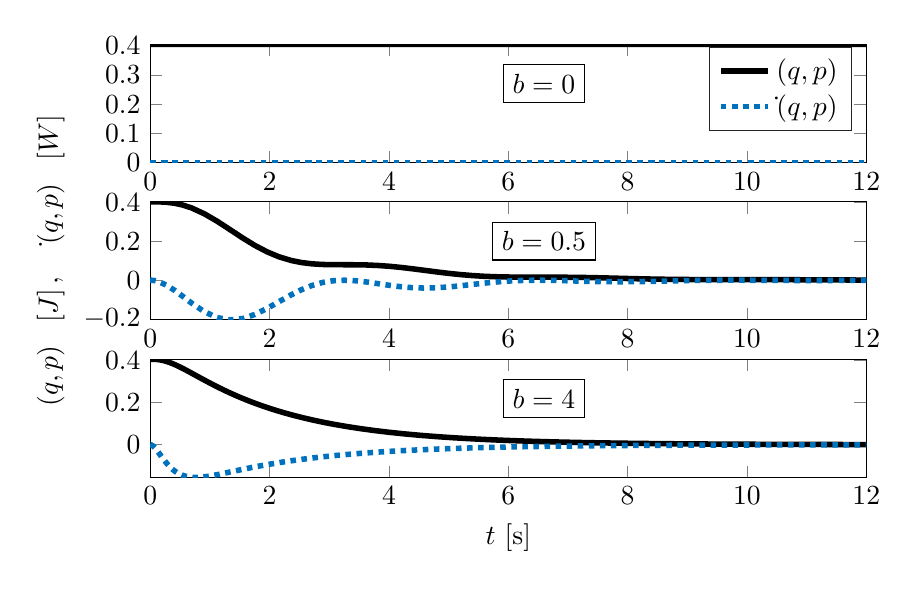
\begin{tikzpicture}

\begin{axis}[%
width=0.75\linewidth,
height=1.5cm,
at={(1.124in,10cm)},
scale only axis,
xmin=0,
xmax=12,
ymin=0,
ymax=0.405177711238185,
%title={$b = 0$},
legend style={legend cell align=left, align=left, draw=white!15!black}
]
\node[draw] at (5cm,1cm) {$b = 0$};
\addplot [color=black, line width=2.0pt]
  table[row sep=crcr]{%
0	0.405\\
0.00558196984779907	0.405000000000037\\
0.0111639396955981	0.405000000000075\\
0.0167459095433972	0.405000000000033\\
0.0223278793911963	0.404999999999972\\
0.0502377286301916	0.405000000577449\\
0.0781475778691869	0.405000001175547\\
0.106057427108182	0.405000000508656\\
0.133967276347178	0.404999999570472\\
0.273489076266092	0.405008817348559\\
0.413010876185006	0.405017638887384\\
0.55253267610392	0.405008095495705\\
0.692054476022834	0.404995502000948\\
0.882622882851168	0.40505162399289\\
1.0731912896795	0.405105958565201\\
1.26375969650783	0.405048873445136\\
1.45432810333617	0.404978396032439\\
1.66522448061415	0.405080485355381\\
1.87612085789213	0.405177711238185\\
2.08701723517011	0.405077080614858\\
2.29791361244809	0.404957240439046\\
2.49359204877776	0.405022858085592\\
2.68927048510742	0.405086135923666\\
2.88494892143709	0.405019891652357\\
3.08062735776676	0.404938795834016\\
3.29217572928616	0.405042748958118\\
3.50372410080557	0.405141694266096\\
3.71527247232497	0.405039336701893\\
3.92682084384437	0.404917594179105\\
4.12394370956561	0.404986118972774\\
4.32106657528686	0.405052125179049\\
4.5181894410081	0.40498309589074\\
4.71531230672934	0.404898798510326\\
4.92804917914053	0.405006229594616\\
5.14078605155172	0.405108380110615\\
5.35352292396291	0.405002806511212\\
5.5662597963741	0.404877530753331\\
5.76496475773265	0.404949361384387\\
5.96366971909119	0.405018464974297\\
6.16237468044974	0.404946278910651\\
6.36107964180828	0.404858367134985\\
6.57522767025033	0.404970053434698\\
6.78937569869237	0.405076119292893\\
7.00352372713441	0.404966623013104\\
7.21767175557645	0.404837055187637\\
7.41804847500585	0.404912521096047\\
7.61842519443524	0.404985024579151\\
7.81880191386464	0.40490937930336\\
8.01917863329403	0.404817524209702\\
8.22835222657444	0.404914756751895\\
8.43752581985484	0.405007493781065\\
8.64669941313525	0.404911379610052\\
8.85587300641565	0.404796538443848\\
9.05730825802623	0.404874380706413\\
9.2587435096368	0.404949103200885\\
9.46017876124737	0.404871203514256\\
9.66161401285794	0.404776788322777\\
9.86314170214268	0.40485483786999\\
10.0646693914274	0.40492975371553\\
10.2661970807122	0.404851657794485\\
10.4677247699969	0.404757020358642\\
10.6697989726996	0.404836323673505\\
10.8718731754022	0.404912409094004\\
11.0739473781048	0.404833126064686\\
11.2760215808075	0.404737143883105\\
11.4570161856056	0.404778485302241\\
11.6380107904037	0.404818793251919\\
11.8190053952019	0.40477617483988\\
12	0.404722769265542\\
};
\addlegendentry{$\Ha(q,p)$}

\addplot [color=ocean, dotted, line width=2.0pt]
  table[row sep=crcr]{%
0	0\\
0.00558196984779907	0\\
0.0111639396955981	0\\
0.0167459095433972	0\\
0.0223278793911963	0\\
0.0502377286301916	0\\
0.0781475778691869	0\\
0.106057427108182	0\\
0.133967276347178	0\\
0.273489076266092	0\\
0.413010876185006	0\\
0.55253267610392	0\\
0.692054476022834	0\\
0.882622882851168	0\\
1.0731912896795	0\\
1.26375969650783	0\\
1.45432810333617	0\\
1.66522448061415	0\\
1.87612085789213	0\\
2.08701723517011	0\\
2.29791361244809	0\\
2.49359204877776	0\\
2.68927048510742	0\\
2.88494892143709	0\\
3.08062735776676	0\\
3.29217572928616	0\\
3.50372410080557	0\\
3.71527247232497	0\\
3.92682084384437	0\\
4.12394370956561	0\\
4.32106657528686	0\\
4.5181894410081	0\\
4.71531230672934	0\\
4.92804917914053	0\\
5.14078605155172	0\\
5.35352292396291	0\\
5.5662597963741	0\\
5.76496475773265	0\\
5.96366971909119	0\\
6.16237468044974	0\\
6.36107964180828	0\\
6.57522767025033	0\\
6.78937569869237	0\\
7.00352372713441	0\\
7.21767175557645	0\\
7.41804847500585	0\\
7.61842519443524	0\\
7.81880191386464	0\\
8.01917863329403	0\\
8.22835222657444	0\\
8.43752581985484	0\\
8.64669941313525	0\\
8.85587300641565	0\\
9.05730825802623	0\\
9.2587435096368	0\\
9.46017876124737	0\\
9.66161401285794	0\\
9.86314170214268	0\\
10.0646693914274	0\\
10.2661970807122	0\\
10.4677247699969	0\\
10.6697989726996	0\\
10.8718731754022	0\\
11.0739473781048	0\\
11.2760215808075	0\\
11.4570161856056	0\\
11.6380107904037	0\\
11.8190053952019	0\\
12	0\\
};
\addlegendentry{$\dot{\Ha}(q,p)$}

\end{axis}

\begin{axis}[%
width=0.75\linewidth,
height=1.5cm,
at={(1.124in,8cm)},
scale only axis,
xmin=0,
xmax=12,
ymin=-0.204912881266039,
ymax=0.405,
ylabel={$\Ha(q,p)~~\left[\text{J}\right],~~~\dot{\Ha}(q,p)~~\left[\text{W}\right]$},
legend style={legend cell align=left, align=left, draw=white!15!black}
]
\node[draw] at (5cm,1cm) {$b = 0.5$};
\addplot [color=black, line width=2.0pt]
  table[row sep=crcr]{%
0	0.405\\
0.00558196984779907	0.404999976567903\\
0.0111639396955981	0.404999812947783\\
0.0167459095433972	0.404999370042739\\
0.0223278793911963	0.404998509951744\\
0.0502377286301916	0.404983206037347\\
0.0781475778691869	0.404937495470277\\
0.106057427108182	0.404845544759889\\
0.133967276347178	0.404692322596255\\
0.273516522542154	0.402530852560815\\
0.413065768737131	0.397086011178988\\
0.552615014932108	0.387458219799325\\
0.692164261127084	0.373274028629815\\
0.907269193523539	0.342843381071733\\
1.12237412591999	0.304278629018944\\
1.33747905831645	0.261141987365565\\
1.5525839907129	0.217476404141547\\
1.75422600025637	0.179475405491745\\
1.95586800979984	0.146812653522303\\
2.1575100193433	0.120903356814893\\
2.35915202888677	0.102117468946583\\
2.53381146818428	0.0912597545861774\\
2.70847090748178	0.0846642354070274\\
2.88313034677929	0.0813160247136622\\
3.05778978607679	0.0800891350264095\\
3.25229709785627	0.0798974497802438\\
3.44680440963575	0.0796987799006767\\
3.64131172141523	0.0785079465729382\\
3.8358190331947	0.0757485768675346\\
4.0227142230037	0.0714655958896716\\
4.2096094128127	0.0657305772193612\\
4.39650460262169	0.058903137924015\\
4.58339979243069	0.0514687533485556\\
4.78779223544894	0.0432719083625159\\
4.99218467846718	0.0356462661505543\\
5.19657712148542	0.0290864268560461\\
5.40096956450367	0.0238809705106763\\
5.58272031174094	0.0204696713866693\\
5.76447105897822	0.0181441848254574\\
5.94622180621549	0.016742939819788\\
6.12797255345277	0.016041999941959\\
6.32751523007192	0.0157867170562464\\
6.52705790669108	0.015763909830532\\
6.72660058331024	0.0157003134624063\\
6.92614325992939	0.015402045601961\\
7.11151061116563	0.014824930167094\\
7.29687796240187	0.0139389495205726\\
7.48224531363811	0.0127789352241093\\
7.66761266487435	0.0114184052570543\\
7.87576626103452	0.00977210344780954\\
8.08391985719468	0.00814360371171002\\
8.29207345335485	0.0066601754934905\\
8.50022704951501	0.00541302298276011\\
8.69377185543363	0.00451081779779689\\
8.88731666135224	0.0038646659769947\\
9.08086146727086	0.00345106188562289\\
9.27440627318948	0.00322497224917417\\
9.47733620279232	0.00312864693228089\\
9.68026613239515	0.00310995715722783\\
9.88319606199799	0.00310646692235253\\
10.0861259916008	0.00307033527466572\\
10.3002873334557	0.00296506208217241\\
10.5144486753105	0.0027788681725499\\
10.7286100171654	0.00251847787159385\\
10.9427713590203	0.00220550337549205\\
11.1662986311212	0.00185527617991145\\
11.3898259032222	0.00151604937496107\\
11.6133531753232	0.00121688741078279\\
11.8368804474241	0.000976645804463098\\
11.8776603355681	0.000940047157137025\\
11.9184402237121	0.000905716717419815\\
11.959220111856	0.000873647677976041\\
12	0.000843821433264805\\
};

\addplot [color=ocean, dotted, line width=2.0pt]
  table[row sep=crcr]{%
0	0\\
0.00558196984779907	-1.25838536176011e-05\\
0.0111639396955981	-5.01936587132233e-05\\
0.0167459095433972	-0.000112615486732318\\
0.0223278793911963	-0.000199633711145713\\
0.0502377286301916	-0.000996009586867228\\
0.0781475778691869	-0.00237403757677018\\
0.106057427108182	-0.00430506809848731\\
0.133967276347178	-0.00675965823051534\\
0.273516522542154	-0.0258162900321056\\
0.413065768737131	-0.0532799840581812\\
0.552615014932108	-0.0852049492511642\\
0.692164261127084	-0.117905279077558\\
0.907269193523539	-0.162638961430211\\
1.12237412591999	-0.193128100615591\\
1.33747905831645	-0.204912881266039\\
1.5525839907129	-0.197786172503555\\
1.75422600025637	-0.176689559024567\\
1.95586800979984	-0.146007118297095\\
2.1575100193433	-0.110788357561423\\
2.35915202888677	-0.0758888034074675\\
2.53381146818428	-0.0490674930900976\\
2.70847090748178	-0.0274273492556652\\
2.88313034677929	-0.0120112432532908\\
3.05778978607679	-0.00303292388146039\\
3.25229709785627	-4.69029382528931e-06\\
3.44680440963575	-0.00291734664518016\\
3.64131172141523	-0.00981333689427549\\
3.8358190331947	-0.0185968351071121\\
4.0227142230037	-0.0270230015663529\\
4.2096094128127	-0.0340171960198438\\
4.39650460262169	-0.0386321083268686\\
4.58339979243069	-0.0404181936218492\\
4.78779223544894	-0.0391526055208492\\
4.99218467846718	-0.0350367485998782\\
5.19657712148542	-0.0289448737918535\\
5.40096956450367	-0.0219048752443281\\
5.58272031174094	-0.0156639995101443\\
5.76447105897822	-0.0100715941169794\\
5.94622180621549	-0.00556081103647257\\
6.12797255345277	-0.00236941173971474\\
6.32751523007192	-0.000444027064203728\\
6.52705790669108	-2.21109238939862e-05\\
6.72660058331024	-0.000774124398020632\\
6.92614325992939	-0.00227473551075722\\
7.11151061116563	-0.00395345144885526\\
7.29687796240187	-0.00557361792062262\\
7.48224531363811	-0.00687936867184007\\
7.66761266487435	-0.00770491053440868\\
7.87576626103452	-0.00797244748170779\\
8.08391985719468	-0.00756751180088736\\
8.29207345335485	-0.00661867785017754\\
8.50022704951501	-0.00532001179724322\\
8.69377185543363	-0.00398880027445289\\
8.88731666135224	-0.00270739722909454\\
9.08086146727086	-0.00160742930090221\\
9.27440627318948	-0.000774361226149226\\
9.47733620279232	-0.000228345543622493\\
9.68026613239515	-9.20974133156524e-06\\
9.88319606199799	-6.36899161288233e-05\\
10.0861259916008	-0.000310464666550314\\
10.3002873334557	-0.000678590759568096\\
10.5144486753105	-0.00105584564504542\\
10.7286100171654	-0.00135898674529172\\
10.9427713590203	-0.00153598356723505\\
11.1662986311212	-0.0015654728161328\\
11.3898259032222	-0.00144700120539884\\
11.6133531753232	-0.00121686752738458\\
11.8368804474241	-0.000925258100009114\\
11.8776603355681	-0.000869652600330071\\
11.9184402237121	-0.000814068554655878\\
11.959220111856	-0.000758797335391599\\
12	-0.000704117867209609\\
};

\end{axis}

\begin{axis}[%
width=0.75\linewidth,
height=1.5cm,
at={(1.124in,6cm)},
scale only axis,
xmin=0,
xmax=12,
xlabel={$t$ [s]},
ymin=-0.154695651812255,
ymax=0.405,
%ylabel={$\Ha(q,p),~\dot{\Ha}(q,p)$},
%title={$b = 4$},
legend style={legend cell align=left, align=left, draw=white!15!black}
]
\node[draw] at (5cm,1cm) {$b = 4$};
\addplot [color=black, line width=2.0pt]
  table[row sep=crcr]{%
0	0.405\\
0.00558196984779907	0.404999815375109\\
0.0111639396955981	0.404998546766085\\
0.0167459095433972	0.404995175683795\\
0.0223278793911963	0.404988752136697\\
0.0502377286301916	0.404882374756938\\
0.0781475778691869	0.404590730810983\\
0.106057427108182	0.404053600595832\\
0.133967276347178	0.403234853286679\\
0.179440547360678	0.401258086757921\\
0.224913818374177	0.398468512813394\\
0.270387089387677	0.394900097815955\\
0.315860360401177	0.390631187053873\\
0.369029285415253	0.38487841094929\\
0.42219821042933	0.378424890863502\\
0.475367135443406	0.371402158886722\\
0.528536060457482	0.363947648763725\\
0.591096534120729	0.354789283716206\\
0.653657007783976	0.345338180621557\\
0.716217481447223	0.335713436061063\\
0.77877795511047	0.326029180801431\\
0.851924754753838	0.314752245553419\\
0.925071554397207	0.303595546690981\\
0.998218354040575	0.292622926086128\\
1.07136515368394	0.281896237554506\\
1.15855954304823	0.269491363986806\\
1.24575393241252	0.257515836495894\\
1.3329483217768	0.245982845577749\\
1.42014271114109	0.234909769716187\\
1.52633017303552	0.222054834241416\\
1.63251763492995	0.209862005777584\\
1.73870509682438	0.198305886909937\\
1.84489255871881	0.187369761360648\\
1.97785432307526	0.174517095687552\\
2.1108160874317	0.162534067779958\\
2.24377785178815	0.15136261528964\\
2.3767396161446	0.140955877170447\\
2.54959694037553	0.128492810355519\\
2.72245426460646	0.117128333409301\\
2.89531158883739	0.106764217243126\\
3.06816891306832	0.0973171261096022\\
3.29863326754768	0.0860148079445944\\
3.52909762202704	0.0760229165536791\\
3.7595619765064	0.0671868148277369\\
3.99002633098576	0.059378587536235\\
4.26563662642477	0.0512355883178454\\
4.54124692186377	0.0442037639754037\\
4.81685721730277	0.0381228242274728\\
5.09246751274177	0.0328818453175525\\
5.2841684444337	0.0296781475121151\\
5.47586937612562	0.0267834930829467\\
5.66757030781754	0.0241658904473271\\
5.85927123950947	0.0218044858791771\\
6.05097217120139	0.0196780327760519\\
6.24267310289331	0.0177578577554488\\
6.43437403458524	0.0160231759664426\\
6.62607496627716	0.0144580803970437\\
6.86216583796056	0.0127416106971852\\
7.09825670964396	0.011227994183285\\
7.33434758132737	0.00989206640111069\\
7.57043845301077	0.00871547894311384\\
7.83957358098027	0.007548792499022\\
8.10870870894977	0.00653619282418212\\
8.37784383691928	0.00565412001730241\\
8.64697896488878	0.00489231667788266\\
8.84084714252195	0.00441207833768404\\
9.03471532015512	0.00397778719851583\\
9.22858349778829	0.00358416684079671\\
9.42245167542146	0.00322966029171595\\
9.61631985305463	0.00291191506617544\\
9.8101880306878	0.00262498059852476\\
10.004056208321	0.0023655372026725\\
10.1979243859541	0.0021317977535099\\
10.4326656224789	0.00188053239456577\\
10.6674068590037	0.00165850672937192\\
10.9021480955285	0.0014618397202912\\
11.1368893320532	0.00128864801469488\\
11.3526669990399	0.00114850144103926\\
11.5684446660266	0.00102331012133229\\
11.7842223330133	0.000911177027288633\\
12	0.000811414399458198\\
};

\addplot [color=ocean, dotted, line width=2.0pt]
  table[row sep=crcr]{%
0	0\\
0.00558196984779907	-9.87271751477061e-05\\
0.0111639396955981	-0.000386225018995059\\
0.0167459095433972	-0.000849950563050964\\
0.0223278793911963	-0.00147798138690459\\
0.0502377286301916	-0.00670595068954835\\
0.0781475778691869	-0.0145647203774138\\
0.106057427108182	-0.0241143214589477\\
0.133967276347178	-0.0346412658980975\\
0.179440547360678	-0.0525657732189105\\
0.224913818374177	-0.0701212813655781\\
0.270387089387677	-0.0863701863346054\\
0.315860360401177	-0.100855324478731\\
0.369029285415253	-0.115347833381428\\
0.42219821042933	-0.127150364043545\\
0.475367135443406	-0.136406276504761\\
0.528536060457482	-0.143410885729709\\
0.591096534120729	-0.149219868372836\\
0.653657007783976	-0.152767909588319\\
0.716217481447223	-0.154453074210226\\
0.77877795511047	-0.154695651812255\\
0.851924754753838	-0.153628554588499\\
0.925071554397207	-0.151410355014675\\
0.998218354040575	-0.148333911666115\\
1.07136515368394	-0.144692262955801\\
1.15855954304823	-0.139925634965703\\
1.24575393241252	-0.134837708055522\\
1.3329483217768	-0.129570123456121\\
1.42014271114109	-0.124278950062036\\
1.52633017303552	-0.117960750830108\\
1.63251763492995	-0.111797000563839\\
1.73870509682438	-0.105823583898826\\
1.84489255871881	-0.100103737939751\\
1.97785432307526	-0.0933535859745871\\
2.1108160874317	-0.0870105159316328\\
2.24377785178815	-0.0810534614762815\\
2.3767396161446	-0.0754917160486311\\
2.54959694037553	-0.0688436636495038\\
2.72245426460646	-0.0627675271094175\\
2.89531158883739	-0.0572085100771072\\
3.06816891306832	-0.0521416531426631\\
3.29863326754768	-0.0461011117943746\\
3.52909762202704	-0.0407514012349237\\
3.7595619765064	-0.0360025255829317\\
3.99002633098576	-0.0318104906687393\\
4.26563662642477	-0.0274839510682223\\
4.54124692186377	-0.023723554464252\\
4.81685721730277	-0.0204204129919938\\
5.09246751274177	-0.0175908399649661\\
5.2841684444337	-0.0158998619286253\\
5.47586937612562	-0.014359013757335\\
5.66757030781754	-0.0129463295886782\\
5.85927123950947	-0.0116741247309791\\
6.05097217120139	-0.0105437838112004\\
6.24267310289331	-0.00951846740062228\\
6.43437403458524	-0.00858532199627462\\
6.62607496627716	-0.0077441910868652\\
6.86216583796056	-0.00683103425597194\\
7.09825670964396	-0.00602182324069\\
7.33434758132737	-0.00529994656565538\\
7.57043845301077	-0.0046661592628758\\
7.83957358098027	-0.00405507699332014\\
8.10870870894977	-0.00351559942337489\\
8.37784383691928	-0.00302660448632308\\
8.64697896488878	-0.0026104956039012\\
8.84084714252195	-0.00236301286907971\\
9.03471532015512	-0.00213418706366242\\
9.22858349778829	-0.00191919622306412\\
9.42245167542146	-0.00172650998189649\\
9.61631985305463	-0.00155995774774332\\
9.8101880306878	-0.0014076645111795\\
10.004056208321	-0.00126710183571991\\
10.1979243859541	-0.00114082000735059\\
10.4326656224789	-0.00100888214221419\\
10.6674068590037	-0.000890691614164208\\
10.9021480955285	-0.00078291861709471\\
11.1368893320532	-0.000688798852963226\\
11.3526669990399	-0.00061587724736729\\
11.5684446660266	-0.000549523565729055\\
11.7842223330133	-0.000487961658165162\\
12	-0.000433625652401622\\
};
\end{axis}

\end{tikzpicture}%
        \caption[Time evolution of the Energy of the mass--spring damper system.]{Time evolution of the Energy and its time derivative for the mass--spring damper system. When $b=0$, the energy is conserved. When $b\neq 0$, the energy is dissipated as the system's state reaches its minimum. By increasing the value of the damping coefficient, the energy dissipation rate becomes more uniform as $\dot{\Ha}$ has a less oscillations. Mote that the convergence time in the cases $b = 0.5$ and $b = 4$ is comparable.}
        \label{fig:msd_en}
        %
    \end{figure}
    %
\end{exmp}
%
%
\begin{exmp}[Lotka--Volterra equations]
    The classical formulation of the LV model is the following autonomous dynamical system:
    %
    \begin{equation}\label{eq:lv}
        \left\{ 
            \begin{matrix*}[l]
                \dot{\xi} = a\xi - b\xi\eta\\
                \dot{\eta} = -c\eta + d\xi\eta
            \end{matrix*}\right.
    \end{equation}
    %
    where $\xi(t)$, $\eta(t)\in\R$ represent the time evolution of the populations of prey and predators, respectively. The positive parameters $a$, $b$, $c$, and $d$ have the following meaning:
    %
    \begin{itemize}
        \item [$a$:] Natural growth rate of the prey in absence of predators;
        \item [$b$:] effect of predation on the prey
        \item [$c$:] natural death rate of the predators in absence of prey
        \item [$d$:] efficiency and propagation rate of the predators in the presence of prey.
    \end{itemize}
    %
    The Lotka--Volterra model has the structure of a canonical Hamiltonian system \citep{vulpiani2010chaos}. 
    Let us divide the two equations in (\ref{eq:lv}) by $\xi$ and $\eta$, respectively, and $(q,p)\triangleq(\ln(\xi),\ln(\eta))$. This leads to
	%
	\begin{equation*}
	    \left\{ 
	        \begin{matrix*}[l]
	            \dfrac{\dot{\xi}}{\xi} = a - b\eta\\
	            \dfrac{\dot{\eta}}{\eta} = -c + d\xi
	        \end{matrix*}\right.
    \Leftrightarrow
    \left\{ 
	\begin{matrix*}[l]
	\dot{q} = -c + de^p = \dfrac{\partial}{\partial p}(-cp+de^p + \gamma(q))\\
	\dot{p} = a - be^q = -\dfrac{\partial}{\partial q}(-aq+be^q + \mu(p))
	\end{matrix*}\right.
	\end{equation*}
	%
	\text{for any scalar functions $\gamma(q)$ and $\mu(p)$}. Selecting 
	\begin{equation}
	    \gamma(q) = aq-be^q,~~ \mu(p) = -cp+de^p   
	\end{equation}
	%
	yields
	%
	\begin{equation*}
	\left\{ 
	\begin{matrix*}[l]
	\dot{q}  = \dfrac{\partial}{\partial p}(-cp + de^p - aq +be^q) =  {\nabla}_{p}\Ha\\
	\dot{p}  = -\dfrac{\partial}{\partial q}(-cp + de^p - aq +be^q) =  -{\nabla}_{q}\Ha
	\end{matrix*}\right.
	\end{equation*}
	%
	and, consequently, the Hamiltonian function results in
	%
	\begin{equation}
	\Ha(q,p) = -aq + be^q - cp +de^p.
	\end{equation}
	%
	The final port--Hamiltonian model is
	\begin{equation}\label{eq:LVph}
	\left\{
	\begin{matrix*}[l]
	%%
	\begin{bmatrix}	\dot{q}\\\dot{p}\end{bmatrix} 
	=
	%
	\begin{bmatrix}0&1\\-1&0\end{bmatrix}
	%
	\begin{bmatrix}{\nabla}_{q}\Ha\\{\nabla}_{p}\Ha\end{bmatrix}
	+
	\mathbf{G}(q,p)\ub\\
	%%
	\yb = \mathbf{G}^\top(q,p)\begin{bmatrix}{\nabla}_{q}\Ha\\{\nabla}_{p}\Ha\end{bmatrix}
	\end{matrix*}
	\right.
	\end{equation}
	%
	Note that the Lotka--Volterra system is lossless, i.e. the variation of $\Ha$ is solely due to the injected (extracted) power:
	%
	\begin{equation}
	    \dot{\Ha}(\xb) = \yb^\top\ub
	\end{equation}
	%
	In the case of classical mechanics, the Hamiltonian function physically represents the total energy of the system. In this case, it simply reflects the ``conserved quantity''. Moreover, it is not clear by first principles what inputs and outputs should be. In practice, they would depend on how it is possible to influence the biological system; 
\end{exmp}
%
\begin{figure}[!ht]
    \centering
    %\tikzstyle{block} = [draw, fill=gray!20, rectangle, 
minimum height=1em, minimum width=2em]
\tikzstyle{sum} = [draw, fill=gray!50, circle, node distance=1cm]
\tikzstyle{input} = [coordinate]
\tikzstyle{output} = [coordinate]
\tikzstyle{pinstyle} = [pin edge={to-,thin,black}]
\tikzset{container/.style={draw, rectangle, dashed, inner sep=1.7em }}
	% The block diagram code is probably more verbose than necessary
	\begin{tikzpicture}[auto, node distance=2cm,>=latex']
	% We start by placing the blocks
	\node [input](input){};
	\node [sum, right of=input, node distance= 60] (sum) {};
	\node [block, right of=sum] (int) {$\int$};
	\node [block,right of = int](log1){$e^{(\cdot)}$};
    \node [output, right of=log1] (output) {};
    
    %
    \node [block, name=G,below of = input,  node distance = 45] {\begin{tabular}{|l|}\hline
        $\mathbf{G}_{11}~\cdots~\mathbf{G}_{1m}$ \\\hline
        $\mathbf{G}_{21}~\cdots~\mathbf{G}_{2m}$ \\\hline
    \end{tabular}};
    \node [input,left of=G, node distance= 60,name=u]{};
    %\node [block, name=G1,below of = input,  node distance = 29.5] {$\mathbf{G}_1(q,p)$};
    %\node [block, name=G2,below of = G1,  node distance = 15.5] {$\mathbf{G}_2(q,p)$};
    
	\node [block, below of=int,node distance = 30] (dq) {$a-be^{(\cdot)}$};
	\node [block, below of = dq, node distance = 30] (dp) {$-c+de^{(\cdot)}$};
	%
    
    \node[block,below of=dp, node distance = 30](int2) {$\int$};
	\node [sum, below of=sum, node distance = 90] (sum2) {};
	\node [input, name=input2,below of = input,  node distance = 90] {};
    \node [block,right of = int2](log2){$e^{(\cdot)}$};
	\node [output, right of=log2] (output2) {};
    
	\node [output, right of=int2, node distance = 37.5] (y3) {};
	\node [output, right of=int, node distance = 37.5] (y1) {};
	\node [output, right of=sum2, node distance = 29.5] (y4) {};
    
	% Once the nodes are placed, connecting them is easy. 
	\draw [draw,-latex] (u) -- node {$\mathbf{u}$} (G);
	\draw [draw,-latex] (G.10) to[out = 0, in = 180] (sum);
	\draw [draw,-latex] (G.350) to[out = 0, in = 180] (sum2);
	
	\draw [-latex] (sum) -- node {$\dot{q}$} (int);
	\draw [-latex] (sum2) -- node {\vspace*{100mm} $\dot{p}$} (int2);
	
	\draw [-latex] (int) -- node [name=y] {$q$}(log1);
	\draw [-latex] (int2) -- node [name=y2] {$p$}(log2);
    \draw [-latex] (log1) -- node [name=y5] {\hspace{10mm} $\eta$}(output);
	\draw [-latex] (log2) -- node [name=y6] {\hspace{10mm} $\xi$}(output2);
    
	\draw [-latex] (y1) |- (dq);
	\draw [-latex] (y3) |- (dp);
	%\draw [-latex] (dq.west) -- node[] {} 
	%node [near end] {} (sum2);
	\draw [-latex] (dq.west) to[out = 180, in = 45] (sum2);
	\draw [-latex] (dp.west) to[out = 180, in = -45] (sum);
    
	\draw  node [below of = sum, node distance = 0] (p1) {$+$};
	\draw  node [below of = sum2, node distance = 0] (p2) {$+$};
\end{tikzpicture}
    \caption[Block diagram representation of the Lotka--Volterra equations in port--Hamiltonian form.]{Block diagram representation of the Lotka--Volterra equations in port--Hamiltonian form. The diagram is obtained from equation (\ref{eq:LVph}).}
    \label{fig:LVscheme}
\end{figure}
%
Up to this point, we have seen the generality of port--Hamiltonian systems showing how they can be used to model both physical systems (from first principles) and purely mathematical dynamics. In the following, the basic notions of passivity--based--control (PBC) and the \textit{energy--balancing} PBC technique will be discussed. 
%
%%%%%%%%%%%%%%%%%%%%%%%%%%%%%%%%%%%%%%
\subsection{Passivity--Based Control}
%
As pointed out in the previous part, any local minimum of the energy is a (locally) stable equilibrium point of the system. Thus, it is intuitive to understand how the \textit{shape} of the energy function is always related to stability properties. 
In the framework passivity--based control of port--Hamiltonian systems, controllers are aimed at modify the closed--loop energy function of the plant by changing its \textit{shape} to obtain the desired stability property, e.g. shift the minimum of the energy into a desired set point. This approach is referred to as ``energy shaping control''. The energy shaping control problem is hereafter formally introduced.
%
\begin{prob}[Passivity--based control]
Consider a PH system (\ref{eq:PHsys}). A control action $\ub = \bm\beta(\xb) + \mathbf{v}$ solves the PBC problem if the closed--loop system satisfies a desired power--balance equation
%
\begin{equation*}
	\dot{\Ha}^*(\xb)
	= \zb^\top \vb - d^*
\end{equation*}
where $\Ha^*(\xb)$ is the desired energy function, $d^*$ the desired dissipation function and $\zb\in\R^m$ the new power conjugated (passive) output.
\end{prob}
%
The most common solution to the PBC problem is the \textit{energy--balancing PBC} (EB--PBC) proposed by \cite{ortega2000}. Roughly speaking, the controller is obtained directly from the power balance equation by setting the desired dissipation $d^*$ equal to the natural dissipation of the system, i.e,
%
\begin{equation}
    d^* \triangleq \bm\nabla^\top\Ha(\xb)\mathbf{R}(\xb)\bm\nabla\Ha(\xb)
\end{equation}
%
and keeping the same output 
%
\begin{equation}
    \zb \triangleq \yb.
\end{equation}
%
Next proposition gives an operative insight of how to accomplish the EB--PBC control task
%
\begin{prop}[\citealp{secchi2007control}]\label{prop:ebpbc}
If it is possible to find a function $\bm\beta(\xb)$ such that
\begin{equation}
    \dot{\Ha}_a(\xb)
    =-\yb^\top\bm\beta(\xb)
\end{equation}
then the control law $\ub = \bm\beta(\xb)+\vb$ is such that 
\begin{equation}
    \dot{\Ha}^*(\xb)
    = \yb^\top \vb -d^*
\end{equation}
is satisfied for $\Ha^*(\xb) \triangleq \Ha(\xb)+\Ha_a(\xb)$.
\end{prop}
This implies that the state feedback $\bm\beta(\xb)$ is such that the \textit{added energy} $\Ha_a$ equals the energy supplied to the system and, consequently, $\Ha^*$ is the difference between the stored and supplied energy.
%
\newline

%
In  \citep{ortega2008control} the closed-form solution of the EB--PBC controller is given by 
%
\begin{equation}\label{eq:ebpbc}
    \bm\beta(\xb) = -\left(\mathbf{G}^{\top}(\xb)\mathbf{G}(\xb)\right)^{-1}\mathbf{G}^{\top}(\xb)\left[\mathbf{J}(\xb)-\mathbf{R}(\xb)\right]^\top\bm\nabla\Ha_a(\xb)
\end{equation}
%
where $\Ha_a$ satisfies the following matching equations 
%
\begin{equation}
    \begin{bmatrix}\mathbf{G}^{\perp}\left[\mathbf{J}-\mathbf{R}\right]^\top\\\mathbf{G}^\top\end{bmatrix}\bm\nabla\Ha_a(\xb) = \mymathbb{0}_{n+m}
\end{equation}
%
being $\mathbf{G}^{\perp}$ a left full--rank annihilator of $\mathbf{G}$.

The idea behind this state--feedback control is to ``shape'' the energy function so that its minima translates towards a new minimum, representing the desired working condition of the controlled system (e.g. \textit{PD + gravity compensation} in robot regulation, \cite{arimoto1984stability, secchi2007control}).

The closed--loop system might still be rewritten in port--Hamiltonian form as
%
\begin{equation}\label{eq:PHsys_ctrl}
	\left\{
	    \begin{matrix*}[l]
	        \dot{\xb} = \left[\mathbf{J}(\xb) - \mathbf{R}(\xb)\right]\bm{\nabla}\Ha^*(\xb) + \mathbf{G}(\xb)\mathbf{v}\\
	        \mathbf{y} = \mathbf{G}^\top(\xb)\bm{\nabla}\Ha^*(\xb) 
	    \end{matrix*}
	\right..
\end{equation}
%
Furthermore, it is worth to be noticed that the control law 
\begin{equation}\label{eq:damping}
    \mathbf{v}\triangleq -\mathbf{K}_{d}\yb,~~~~(\mathbf{K}_d = \mathbf{K}_d^\top \succ 0)
\end{equation}
%
asymptotically stabilizes the minima of $\Ha^*(\xb)$. This negative output feedback law is usually referred to as \textit{damping injection}. Reasoning in a physical manner, the control law (\ref{eq:damping}) behaves as an \textit{dissipative} element, contributing to the {energy dissipation} together to matrix $\mathbf{R}(\xb)$. In fact,
%
\begin{align}
    \dot{\xb} &= \left[\mathbf{J}(\xb) - \mathbf{R}(\xb)\right]\bm{\nabla}\Ha^*(\xb) + \mathbf{G}(\xb)\mathbf{v} \\
    &= \left[\mathbf{J}(\xb) - \mathbf{R}(\xb)\right]\bm{\nabla}\Ha^*(\xb) - \mathbf{G}(\xb)\mathbf{K}_{d}\yb\\
    &= \left[\mathbf{J}(\xb) - \mathbf{R}(\xb)\right]\bm{\nabla}\Ha^*(\xb) - \mathbf{G}(\xb)\mathbf{K}_{d}\mathbf{G}^\top(\xb)\bm{\nabla}\Ha^*(\xb)\\
    &=\left[\mathbf{J}(\xb) - \left(\mathbf{R}(\xb) + \mathbf{G}(\xb)\mathbf{K}_{d}\mathbf{G}^\top(\xb)\right)\right]\bm{\nabla}\Ha^*(\xb) 
\end{align}
and $\mathbf{G}(\xb)\mathbf{K}_{d}\mathbf{G}^\top(\xb)\succeq 0$.
%
\begin{rem}
    Generally speaking, the design of an EB--PBC Controller might be nontrivial. In fact, it is needed to find such a $\bm\beta(\xb)$ which guarantees the solvability of the following partial differential equation
    \begin{equation}
        \bm\nabla^\top \Ha_a(\xb)\left[\left[\mathbf{J}(\xb)-\mathbf{R}(\xb)\right]\bm\nabla\Ha(\xb) + \mathbf{G}(\xb)\bm\beta(\xb)\right] = -\mathbf{G}^\top(\xb)\bm\nabla\Ha_a(\xb)\bm\beta(\xb)
    \end{equation}
\end{rem}
%
Few practical examples of the EB--PBC will be given hereafter.
%
\begin{exmp}[Fully--actuated mechanical system]
    Consider the model (\ref{eq:nDOF}) discussed in Example \ref{ex:ndof} and let $\qb^*$ be a desired configuration of the system. A possible choice of $\bm\beta(\qb)$ which satisfies the conditions given by Proposition \ref{prop:ebpbc} is
    %
    \begin{equation}
        \bm\beta(\xb) = \mathbf{B}^{-1}(\qb)\left[\bm\nabla_{\qb}\V(\q) - \bm\nabla_\qb\Ha_a(\qb,\pb)\right]
    \end{equation}
    %
    with $\Ha_a(\qb,\pb)$ having a minimum is $\qb^*$. This control action ``cancels'' the potential $\V(\qb)$ and introduces a new potential $\Ha_a(\qb,\pb)$. A simple choice is a spring--like potential, i.e.
    %
    \begin{equation}
        \Ha_a(\qb,\pb) = \left(\qb-\qb^*\right)^\top\mathbf{K}_p\left(\qb-\qb^*\right),~~~~\mathbf{K}_p = \mathbf{K}_p^\top\succ 0
    \end{equation}
    %
    Thus, including the damping injection action $\vb = -\mathbf{K}_d\yb =-\mathbf{K}_d\mathbf{B}^\top\dot{\qb}$, the control law becomes:
    %
    \begin{equation}
        \bm\beta(\xb) = \mathbf{B}^{-1}(\qb)\left[\bm\nabla_{\qb}\V(\q) - \mathbf{K}_p\left(\qb-\qb^*\right)\right] - \mathbf{K}_d\mathbf{B}^\top\dot{\qb}
    \end{equation}
    %
    %
\end{exmp}
%
The EB-PBC will then be applied to the mass--spring--damper of Example \ref{ex:msd} to show some numerical insights. 
%
\begin{exmp}[Mass--spring--damper system]
    Consider the mass--spring--damper model (\ref{eq:msd}) of Example \ref{ex:msd}. We want to apply the control law (\ref{eq:ebpbc}).  Let us set the desired energy function to 
    %
    \begin{equation}
        \Ha^*(q,p)\triangleq \frac{1}{2}\left(\frac{1}{m}p + k_p\left(q-q^*\right)^2\right)
    \end{equation}
    %
    where $q^*$ is a desired set point. It holds,
    %
    \begin{equation}
        \Ha_a = \Ha^* - \Ha = \frac{1}{2}k_p\left(q-q^*\right)^2 - kq^2~\Rightarrow~\bm\nabla\Ha_a = \left[k_p(q-q^*) - kq,\dfrac{p}{m}\right]^\top
    \end{equation}
    %
    and, therefore,
    %
    \begin{align}
        \beta(q) &= -[0,1]\begin{bmatrix}0&-1\\1&-b\end{bmatrix}\begin{bmatrix}k_p(q-q^*) - kq\\\dfrac{p}{m}\end{bmatrix}\\
                 &= -k_p(q-q^*) + kq. 
    \end{align}
    %
    By adding the damping injection term, the total control input becomes
    %
    \begin{equation}
        u = -k_p(q-q^*) + kq - k_d\dot{q}
    \end{equation}
    %
    A numerical simulation has been performed with $m = 1\text{Kg}$, $k = 1\text{N}\cdot\text{m}^{-1}$, $b = 0.5\text{N}\cdot(\text{m}\cdot\text{s})^{-1}$, $k_p = 1$, $q^* = 0.5$, $k_d = 4$ and $[q_0,p_0] = [-0.9,0]$. The state--space trajectory is reported in Figure \ref{fig:ebpbc}. It can be noticed how the minimum of the energy function is shifted to $[q^*,0]^\top$ and how the damping injection allow a more ``direct'' convergence toward the minimum.
    %
    \begin{figure}[!ht]
        \centering
        %\definecolor{ocean}{rgb}{0.00000,0.44700,0.74100}
%
\begin{tikzpicture}
\begin{axis}[
width=5.5cm,
height=5.5cm,
at={(1in,0.331in)},
view={0}{90},
colorbar horizontal,
%colormap/blackwhite,
colormap = {whiteblack}{color(0cm)  = (white);color(1cm) = (black)},
xmin=-1,
xmax=1,
xlabel style={at = {(0.5,-0.1)}},
xlabel={$q(t)~[\text{m}]$},
ymin=-1,
ymax=1,
ylabel style={at = {(-0.1,0.5)}},
ylabel={$p(t)~~[\text{Kg}\cdot\text{m}\cdot\text{s}^{-1}]$},
title = {uncontrolled},
]
\addplot3[contour filled={number = 25,labels={false}},mesh/rows=50,mesh/cols=50,mesh/check=false,forget plot
] table {H.dat};
%
\addplot [color=ocean, line width=1.5pt]
table[row sep=crcr]{%
	-0.9	0\\
	-0.899985991795746	0.00501674269174762\\
	-0.899944019691303	0.0100193471557007\\
	-0.899874162931692	0.0150076971406221\\
	-0.89977650140532	0.0199816771641279\\
	-0.898873958295022	0.0446320420072224\\
	-0.897288646861763	0.0689062780415569\\
	-0.8950312582937	0.0927908195727069\\
	-0.892112845290034	0.116272595485913\\
	-0.868002952216995	0.227228035383425\\
	-0.829223766085857	0.326435243373571\\
	-0.777500187200184	0.412807338237014\\
	-0.714659008971771	0.485603292982159\\
	-0.600340602727355	0.570331414933827\\
	-0.471488130080395	0.621495133714803\\
	-0.335347897263502	0.640176352681101\\
	-0.198445114013884	0.628945422916099\\
	-0.0746437735806325	0.594456994280607\\
	0.0401381420897199	0.540383416283467\\
	0.142232199262124	0.470719359197013\\
	0.229035654600393	0.389586456149254\\
	0.290490142676407	0.313265041426897\\
	0.338339729122556	0.23421079930552\\
	0.372303052526759	0.154991891744638\\
	0.392571550535566	0.0778835525828194\\
	0.399731808807902	-0.00306277450207788\\
	0.391870981971099	-0.0763851640723532\\
	0.370660517667212	-0.14009523114136\\
	0.338087981923116	-0.192856605316552\\
	0.298136191440485	-0.232477962681855\\
	0.25184670416552	-0.260834031598041\\
	0.201350587767438	-0.277964416164619\\
	0.148664452554781	-0.284317405805023\\
	0.0907667653016975	-0.27983068280962\\
	0.0349146831770288	-0.264713991318473\\
	-0.0168257578844223	-0.240602883573134\\
	-0.0628664499768871	-0.20930778888674\\
	-0.0980374609679892	-0.17699717235111\\
	-0.127063690395628	-0.141926700215142\\
	-0.149546840710965	-0.105459101422993\\
	-0.165363769927057	-0.0688391130058303\\
	-0.17517242929207	-0.0298002370528735\\
	-0.177436179549933	0.00664995096132089\\
	-0.172778407588365	0.0393477927721653\\
	-0.162032775025325	0.0674497666527798\\
	-0.147454933577949	0.0889207675276733\\
	-0.129347064906398	0.10558047092737\\
	-0.108623814628922	0.117297644237556\\
	-0.086179982857339	0.124136300367046\\
	-0.0599942658276899	0.126273096752299\\
	-0.03394383333752	0.123024483749271\\
	-0.00911017489546286	0.115053707894857\\
	0.0136390018342169	0.103150490035125\\
	0.0323115311721372	0.0893174145892377\\
	0.0481096403624088	0.0735852869681779\\
	0.0607228554124504	0.0566997231192924\\
	0.0700087283561835	0.0393538111534125\\
	0.0761616883827873	0.0213703319404493\\
	0.0787495703594155	0.00429179247670834\\
	0.0780099609822195	-0.0112862674191978\\
	0.0742949609073913	-0.0249184536659205\\
	0.0676235361779361	-0.0368399446136417\\
	0.0587030242407405	-0.0459531423309749\\
	0.0481558122411435	-0.0521341873494105\\
	0.0365928902454288	-0.0554253293582465\\
	0.0240750228983752	-0.0559548535184\\
	0.0117514398745198	-0.0537959330321324\\
	0.00019941613886286	-0.0493329003279672\\
	-0.0101378207178845	-0.0430176266200058\\
	-0.019073150754024	-0.0351836299097121\\
	-0.0261146445062195	-0.0264793026690255\\
	-0.0311080878005064	-0.0174345850654783\\
	-0.0340432057031742	-0.00851368245135384\\
	-0.0350111008169466	0.000208271867982888\\
	-0.034025886560588	0.00794187081482636\\
	-0.0313546321013023	0.014373201383412\\
	-0.0273270827992865	0.0193247845816726\\
	-0.021776682313328	0.0229649845032737\\
	-0.0155344254822122	0.0247149856554559\\
	-0.00909170615632734	0.0246816915211178\\
	-0.00286371969873624	0.0230947709063524\\
	0.00280725028199055	0.0202496734322155\\
	0.00760795718689828	0.016477401614915\\
	0.0113249300742123	0.0121348606754593\\
	0.0138716616756584	0.00755763965809117\\
	0.0153115070918749	0.00268446415992479\\
	0.0154380718037925	-0.00174353700984352\\
	0.0144046855261442	-0.0054393994641403\\
	0.0124469315254243	-0.00824628912471304\\
	0.00973633834811147	-0.0101436953203082\\
	0.00663307131848225	-0.0109904365212177\\
	0.00344345203354436	-0.010849788231025\\
	0.000418598885933671	-0.00987679726686231\\
	-0.00236889674029977	-0.00817147420768934\\
	-0.00455610701932897	-0.00600636910422985\\
	-0.0060212570956228	-0.00363960519553869\\
	-0.00675662344583174	-0.00129708301418448\\
	-0.00679915540873005	0.000997090639439771\\
	-0.00615806076904666	0.0028415988465903\\
	-0.00499448977320246	0.00409954744618751\\
	-0.00350966028254127	0.0047525483255705\\
	-0.00178742736195878	0.00483753431425414\\
	-0.000142544164199142	0.00436296059647222\\
	0.001233863384226	0.00346409628606365\\
	0.00224352413019931	0.0023187867470898\\
	0.00286423019005585	0.001064908755426\\
	0.00304301781878184	-0.000107287213496858\\
	0.00281783500493549	-0.0010575880234264\\
	0.0022937627777237	-0.00172125518888289\\
	0.00153324548129663	-0.00210115118921709\\
	0.000699028537681449	-0.00212944532957787\\
	-7.39090484163769e-05	-0.00185022451593175\\
	-0.000696860580362937	-0.0013673867011887\\
	-0.00115698870029392	-0.000733929244931739\\
	-0.00134549775988726	-0.000103223462323883\\
	-0.00126431291907824	0.000412349861050412\\
	-0.000993032124110712	0.000759026310963054\\
	-0.000596744297566764	0.000936587972301828\\
	-0.0001714552068425	0.000909680277066964\\
	0.000192405808728558	0.000708505171052146\\
	0.000443835290730197	0.000417655115078066\\
	0.000582041712668234	8.20914139281743e-05\\
	0.000563673850896241	-0.000200244790181628\\
	0.000407680747611572	-0.000363593139831435\\
	0.000193602312173417	-0.000405181279185971\\
	-2.30281468151146e-05	-0.000352938747129361\\
	-0.000186564607289939	-0.000224639431191565\\
	-0.000253723590669539	-6.14216529346211e-05\\
	-0.000236476036563678	7.85096220374468e-05\\
	-0.000162705457701936	0.000174617140937539\\
	-5.64067851445571e-05	0.000196804176492543\\
	4.62570015027289e-05	0.000136732345109551\\
	0.000106953605066236	4.5051528543188e-05\\
	0.00012515523979931	-5.30186446630676e-05\\
	8.69067523052607e-05	-0.000109998447934223\\
	-2.80092519366811e-06	-9.06136603478964e-05\\
	-7.20860461539662e-05	-2.64132971781262e-05\\
	-7.64796094496801e-05	2.09540211186838e-05\\
	-5.84460433855426e-05	5.1911771294405e-05\\
	-2.42154646050572e-05	5.68361010025379e-05\\
	8.96341400149207e-06	4.27250166876023e-05\\
}
[postaction={decorate, decoration={markings,
		mark=between positions 0.4 and 1 step 1 with {\arrow[black,line width=1.5pt]{latex};}
}}]
;
\addplot [color=black, line width=1.0pt, draw=none, mark=*, mark options={solid, fill=red}]
table[row sep=crcr]{%
	0	0\\
};
\end{axis}
%
%
%%%%%%%%%%%%%%%%%%%%%%%%%%%%%%%%%%%%%%%%%%%%%%%%%%%%%%%%%%%%%%%%%%%%%%%%%%%%%%%%%%%%
%%%%%%%%%%%%%%%%%%%%%%%%%%%%%%%%%%%%%%%%%%%%%%%%%%%%%%%%%%%%%%%%%%%%%%%%%%%%%%%%%%%%
%%%%%%%%%%%%%%%%%%%%%%%%%%%%%%%%%%%%%%%%%%%%%%%%%%%%%%%%%%%%%%%%%%%%%%%%%%%%%%%%%%%%
%%%%%%%%%%%%%%%%%%%%%%%%%%%%%%%%%%%%%%%%%%%%%%%%%%%%%%%%%%%%%%%%%%%%%%%%%%%%%%%%%%%%
%%%%%%%%%%%%%%%%%%%%%%%%%%%%%%%%%%%%%%%%%%%%%%%%%%%%%%%%%%%%%%%%%%%%%%%%%%%%%%%%%%%%
%%%%%%%%%%%%%%%%%%%%%%%%%%%%%%%%%%%%%%%%%%%%%%%%%%%%%%%%%%%%%%%%%%%%%%%%%%%%%%%%%%%%
%%%%%%%%%%%%%%%%%%%%%%%%%%%%%%%%%%%%%%%%%%%%%%%%%%%%%%%%%%%%%%%%%%%%%%%%%%%%%%%%%%%%
%%%%%%%%%%%%%%%%%%%%%%%%%%%%%%%%%%%%%%%%%%%%%%%%%%%%%%%%%%%%%%%%%%%%%%%%%%%%%%%%%%%%
%%%%%%%%%%%%%%%%%%%%%%%%%%%%%%%%%%%%%%%%%%%%%%%%%%%%%%%%%%%%%%%%%%%%%%%%%%%%%%%%%%%%
%%%%%%%%%%%%%%%%%%%%%%%%%%%%%%%%%%%%%%%%%%%%%%%%%%%%%%%%%%%%%%%%%%%%%%%%%%%%%%%%%%%%
%
%
\begin{axis}[
width=5.5cm,
height=5.5cm,
at={(3in,0.331in)},
view={0}{90},
colormap = {whiteblack}{color(0cm)  = (white);color(1cm) = (black)},
%point meta max=1,
%point meta min=0,
colorbar horizontal,
xmin=-1,
xmax=1,
xlabel style={at = {(0.5,-0.1)}},
xlabel={$q(t)~[\text{m}]$},
ymin=-1,
ymax=1,
ylabel style={at = {(-0.1,0.5)}},
ylabel={$p(t)~~[\text{Kg}\cdot\text{m}\cdot\text{s}^{-1}]$},
title = {controlled},
]
\addplot3[contour filled={number = 25,labels={false}},mesh/rows=50,mesh/cols=50,mesh/check=false,forget plot
] table {He.dat};
%
\addplot [color=ocean, line width=1.5pt]
  table[row sep=crcr]{%
-0.8	0\\
-0.799990349036801	0.00498033107021971\\
-0.799961618358707	0.0098747291593547\\
-0.799914137292308	0.0146846031489447\\
-0.799848229843306	0.0194113392202208\\
-0.79925339635556	0.0418454401527347\\
-0.79824347460898	0.0623960954334407\\
-0.796853274674598	0.0812122997387488\\
-0.795115141990627	0.0984325323982412\\
-0.790768927263094	0.128296787644992\\
-0.785376036322309	0.153264587331034\\
-0.779105330181172	0.174060070771817\\
-0.772108657930732	0.19133477773411\\
-0.763038186620337	0.208037471054607\\
-0.753289645981645	0.221261670869758\\
-0.74300119403648	0.231602901223056\\
-0.7322979157308	0.239600857080451\\
-0.719261676846459	0.246640822622058\\
-0.705906023060196	0.251536012194579\\
-0.692327192973749	0.254706706027168\\
-0.678614782568464	0.256544729171894\\
-0.66247362618812	0.257426437489457\\
-0.646311874204955	0.257201060461286\\
-0.630183747171902	0.256114775788165\\
-0.61414321680827	0.254412484839407\\
-0.595265767118869	0.25185388221251\\
-0.576596189055644	0.248830613144751\\
-0.558157378273224	0.245463761430925\\
-0.539976790223909	0.241893461361953\\
-0.51817916361628	0.237415489225426\\
-0.496793468063384	0.232827178078682\\
-0.475820890631465	0.228172990928813\\
-0.455270371380758	0.223529646529658\\
-0.430145509394151	0.217814484709777\\
-0.405666363775393	0.21218089737946\\
-0.381817380225226	0.206632931656175\\
-0.358591980971952	0.201211116933391\\
-0.329289992531831	0.194387459270383\\
-0.300983055502358	0.187773986326557\\
-0.273635466117009	0.18135607584414\\
-0.247221432530039	0.17515684728147\\
-0.213216450332404	0.167212672741798\\
-0.180755244907366	0.159612712000165\\
-0.149763118320641	0.152322170089386\\
-0.12018357154267	0.145371602475663\\
-0.0858144492251475	0.137399555625452\\
-0.0533373026575318	0.129810264841887\\
-0.0226270706570543	0.122495986262412\\
0.00636909696235324	0.115634916452806\\
0.0245639001789693	0.11143634041833\\
0.0420958276537119	0.107357005242565\\
0.0589936988963969	0.103373841606505\\
0.0752673828067502	0.0995410710357275\\
0.0909307191540991	0.0958924219558999\\
0.106019132712115	0.0923659165172531\\
0.120555352416888	0.088950524624564\\
0.134555034521067	0.0856623357278251\\
0.151490183124911	0.0817100014164636\\
0.167642971570441	0.0779295655513983\\
0.183052667281672	0.0743001250402007\\
0.197746757068614	0.070844578063958\\
0.214308395158062	0.0670154663998364\\
0.229970491204499	0.0633592974823435\\
0.244794867415063	0.0598130311814775\\
0.25879950337791	0.056490337499804\\
0.268271539243619	0.0543193136019027\\
0.277377664861695	0.0522058138649111\\
0.28613683381004	0.0501280642140806\\
0.294550277212682	0.0481376596317285\\
0.302622660130221	0.046269311168726\\
0.310380814566873	0.0444608841954831\\
0.317839313653139	0.0427005325801324\\
0.325003908428131	0.0410121443424177\\
0.333265108590217	0.0390987513158078\\
0.341139541656519	0.0372608124899314\\
0.348649623182371	0.0354770168477717\\
0.355803058351501	0.0337854742103513\\
0.363392948905419	0.0320649589770333\\
0.370591946577512	0.0303951975475449\\
0.377433707535748	0.0287177788665204\\
0.383907888131925	0.0271577565435242\\
0.389443671632561	0.0259702562002753\\
0.39473090315664	0.0247684358000992\\
0.399801843348943	0.023466122576241\\
0.404620465230478	0.0222660953235561\\
0.408350887799743	0.0214755193934922\\
0.411945686287615	0.0206688588846669\\
0.415417942310123	0.0198136793751198\\
0.418751424695735	0.0190017010518771\\
0.421749435966574	0.0183333261144897\\
0.424640836182413	0.0176712771771757\\
0.427431861811412	0.0170055354392357\\
0.430119184137825	0.016366292811758\\
0.433120168926413	0.0156823501545376\\
0.435994839320273	0.0150160335757382\\
0.43875125849496	0.014355349439579\\
0.44138811564635	0.0137273703851534\\
0.444393641044736	0.0130582638521441\\
0.447250186280145	0.0123997410653497\\
0.449972971893123	0.0117189779650044\\
0.452551926062853	0.0110894822421112\\
0.454986586464819	0.0106126293243617\\
0.457309975238169	0.0100972052264373\\
0.459548116976982	0.00945875119912432\\
0.461660040062453	0.0088972910049626\\
0.463285401817598	0.0086265654600736\\
0.464856320379336	0.00830103919075859\\
0.466390056124709	0.00785944384943798\\
0.467852002939473	0.00746124319329691\\
0.46901908718933	0.00724318304672102\\
0.470150233293014	0.00700366653966192\\
0.471250286391133	0.00672843854962612\\
0.472309341151985	0.00646593652940021\\
0.473385776153833	0.00623606971752866\\
0.474423104615873	0.0060026164567889\\
0.475424864525116	0.00575713819457251\\
0.476386924737601	0.0055236602462727\\
0.477509013526727	0.00528308196053836\\
0.478580917755891	0.00503950426056981\\
0.47960914831749	0.00477550971017029\\
0.480586400027757	0.00453214591275525\\
0.481610040474773	0.00435466654014254\\
0.482588928055224	0.00414391169253402\\
0.483539642880679	0.00384113928384329\\
0.484431987448104	0.00358653847105153\\
0.485149345035107	0.00353796375343561\\
0.4858504258188	0.0034144613798917\\
0.486558116242611	0.00312532124247861\\
0.487221724096408	0.00289337392092469\\
0.487695794885202	0.00286926886972859\\
0.488162830327404	0.00279782215108511\\
0.488630538113274	0.00264914890207623\\
0.489078144940801	0.00251474058075963\\
0.489468942618315	0.00245632917709129\\
0.489849585256036	0.00238252559309817\\
0.490222476966767	0.00228521662647867\\
0.490581431110552	0.00219285824498712\\
0.490983151550325	0.00211716633198077\\
0.491370161570859	0.00203359376410548\\
0.491745602781677	0.00193178322488511\\
0.492103892080372	0.00183846805376174\\
0.492506411397027	0.00178006635551158\\
0.492893660090091	0.00170041146793182\\
0.493274266082875	0.00156719501282182\\
0.493631040787	0.0014580103986811\\
0.49393893278534	0.00148664850092538\\
0.494246737021522	0.00144561045294968\\
0.494576495018397	0.00124452898849242\\
0.494877738115234	0.00110215441053383\\
0.495068936763096	0.00117372907705802\\
0.495268311502121	0.00117249334844865\\
0.495490832327042	0.00103621267596163\\
0.495698067022907	0.000930376939072217\\
0.495840610629077	0.00095247370815219\\
0.495984813415508	0.000944699385649924\\
0.496133828181163	0.000894429628581108\\
0.496277003209635	0.000847895436809127\\
0.496416661006283	0.000836607262138445\\
0.496553688542302	0.000813817356394517\\
0.496690060634777	0.000771984847461256\\
0.496820617308014	0.000733969850716749\\
0.49696822647721	0.000721260119196686\\
0.497112058585325	0.000694991362179336\\
0.497256373125048	0.000638420012584801\\
0.497391864758729	0.000592599260011129\\
0.497516961540873	0.000628416676502535\\
0.497645796617215	0.000617502053678116\\
0.497793169731894	0.000498388425070575\\
0.497924556219102	0.000419921015687774\\
0.497991043928648	0.000459324048068363\\
0.49806207284625	0.000466983808876715\\
0.498141914355139	0.000425154082083012\\
0.498217575709155	0.000389712487736915\\
0.498280352667382	0.000398226266856163\\
0.498343719384198	0.000393641390815707\\
0.498409531198781	0.000368448930993963\\
0.498472348236236	0.000346243263747109\\
0.498539244005894	0.000351289258994947\\
0.498606096029331	0.00034285411516863\\
0.498676569781798	0.000305945207981443\\
0.498742087221458	0.000277766744329463\\
0.498795673719745	0.000323004518209729\\
0.498855674447013	0.000326145795912744\\
0.498934971304551	0.000233034054472018\\
0.499002967777828	0.000174932774746062\\
0.499029744099399	0.000220232876371348\\
0.499062237097782	0.000234908318683179\\
0.49910486552455	0.000200354571654608\\
0.499144513966236	0.000172751063819004\\
0.49917219778251	0.000190647956117142\\
0.499201996901763	0.000194202593015066\\
0.499236023583328	0.000174612949188299\\
0.499268098677856	0.000158436735224372\\
0.499297006810006	0.000174489217785862\\
0.499327973184086	0.000175208410983428\\
0.499364927188323	0.000144141173000527\\
0.499398343871403	0.000122210984435598\\
}
[postaction={decorate, decoration={markings,
		mark=between positions 0.5 and 1 step 1 with {\arrow[black,line width=1.5pt]{latex};}
}}]
;
\addplot [color=black, line width=1.0pt, draw=none, mark=*, mark options={solid, fill=red}]
table[row sep=crcr]{%
	0.5 0\\
};
\end{axis}
\end{tikzpicture}
        \caption[Phase--space trajectory of the mass--spring--damper system control via EB-PBC.]{Phase--space trajectory of the mass--spring--damper system control via EB-PBC. When the EB-PBC control input is applied, the location of the minimum of $\Ha$ is shifted to the desired set point which, in turns, becomes a Lyapunov stable equilibrium of the closed--loop system. Moreover, the dissipation properties are changed via \textit{damping injection}, removing the oscillations during the motion of the system.}
        \label{fig:ebpbc}
    \end{figure}
    %
\end{exmp}
%
\clearpage
%%%%%%%%%%%%%%%%%%%%%%%%%%%%%%%%%%%%%%%%%%%%%%%%%%%%%%%%%%%%%%%%%%%%%%%%%%%%%%%
\section{Hybrid Dynamical Systems\label{sec:HD_systems}}
%
The basic notions of hybrid dynamical system and their hybrid inclusions formulation will be now defined. Part of the content of this Section is inspired by \cite{goebel2009hybrid,Goebel2012}.

Hybrid dynamical systems represent a wide class of systems in which continuous time and discrete time dynamics interacts. In recent years, there has been a growing interest in this field. One of the main reason is that these kind of systems provide a new and promising modeling perspective for systems presenting discontinuous behaviors as well as multimodality. The presence of both discrete and continuous dynamics makes this formalism appealing also for modeling physical phenomena in many different areas, from biology and medical applications to robotics, manufacturing, traffic management and bio-molecular networks~\citep{Aihara4893, Bortolussi2018}. 
Overviews of this framework are given in ~\citep{van2000introduction, haddad2006impulsive,goebel2009hybrid,Goebel2012}.
%
\subsection{Hybrid Inclusions}
%
Hybrid Inclusions are the most general formulation in the hybrid systems framework. They are made up with a constrained differential inclusion and a constrained difference inclusion in the form:
\begin{equation}\label{eq:hs}
%
\left\{ 
\begin{matrix*}[l]\vspace{1pt}
%
\dot{\xb} \in \F(\xb,\ub_c) &&(\xb,\ub_c)\in\C\times\U_c\\
\xb^+ \in \G(\xb,\ub_d)&&(\xb,\ub_d)\in\D\times\U_d
%
\end{matrix*}
\right.
%
\end{equation}
%
with state $\xb\subseteq\R^n$, inputs $\ub_c\in\U_c\subseteq\R^{m_c}$, $\ub_d\in\U_d\subseteq\R^{m_d}$ acting during \textit{flows} and \textit{jumps} respectively. ${\F}:\R^n\times\R^{m_c}\rightrightarrows\R^n$, $\G:\R^n\times\R^{m_d}\rightrightarrows\R^n$ are set--valued mappings and $\C$, $\D$ are subsets of $\R^n$ with. Let us call $\C$ the \textit{flow set}, $\F$ the \textit{flow map}, $\D$ the \textit{jump set} and $\G $ the \textit{jump map}.
%
\newline

%
The trajectories resulting from this kind of systems are defined on a \textit{hybrid time domain}. In fact, given the dual nature of hybrid systems (continuous and discrete), to parametrize its solutions both a continuous time $t$ and an discrete time $k$ are needed.
%
\begin{defn}[Hybrid time domain]
    Let $\E$ be a subset of $\R^+\times\mathbb{N}$, i.e. $\E\subset\R^+\times\mathbb{N}$. $\E$ is a compact hybrid time domain if 
    %
    \begin{equation}
        \E\triangleq\bigcup_{k = 0}^{j-1}\left[t_k,t_{k+1}\right]\times {k} 
    \end{equation}
    %
    such that
    %
    \begin{equation}
        t_0 = 0~~\land~~\forall k\leq j~t_k\leq t_{k+1}~
    \end{equation}
    %
    and one of the following hold:
    \begin{itemize}
        \item [i)] there are infinite intervals, i.e. $j = \infty$;
        \item [ii)] $j<\infty$ and the last interval is of the form
        \begin{equation}
            \left[t_{j-1},t_f\right)\times \{j\}~~\text{with}~~t_f<\infty~\lor~t_f = \infty
        \end{equation}
    \end{itemize}
    %
\end{defn}
%
The solutions of (\ref{eq:hs}) are definite on \textit{hybrid arcs} and parametrized by an hybrid time domain $\E$. The technical details of this formulation are discussed in Appendix \ref{chap:HSapp}. 
%
\begin{exmp}[Bouncing--ball]
\textcolor{red}{to be completed...}
\end{exmp}
%
\begin{exmp}[Elbow prosthesis] 
\textcolor{red}{to be completed...}
\end{exmp}
%
\begin{exmp}[Sliding mode controller]
\textcolor{red}{to be completed...}
\end{exmp}
%
\subsection{Stability}
%
Lyapunov stability theorems has been indeed extended to the hybrid case. In the case of continuous--time dynamical systems, the stability of equilibrium points is usually discussed (see Appendix \ref{chap:stabapp}). However, in case of hybrid systems, it is rather convenient to analyze the stability of a set. Hereafter the very basic results on Lyapunov stability of hybrid systems will be introduced.
%
\begin{thm}[Lyapunov Stability for Hybrid Systems \citep{goebel2009hybrid}]\label{thm:hybrid_Lyap}
	%
	Let us consider an autonomous hybrid system $\left(\C,\F,\D,\G\right)$ and a compact set $\A\subset\R^n$ satisfying $\G\left(\D\cap\A\right)\subset\A$. If there exists a Lyapunov function candidate $V:\C\cup\D\rightarrow\R$ such that:
	\begin{subequations}
		\begin{align}
		&V(\xb)>0&&\forall \xb\in \left(\C\cup\D\right)\setminus\A\label{eq:stabh_1}\\
		&\langle\frac{\partial V}{\partial \xb},\mathbf{f}(\xb)\rangle\leq 0&&\forall \xb\in\C\setminus\A,\mathbf{f}\in\F\label{eq:stabh_2}\\
		&V(\mathbf{g}(\xb)) - V(\xb)\leq 0 &&\forall \xb\in\D\setminus\A,\mathbf{g}\in\G\label{eq:stabh_3}
		\end{align}
	\end{subequations}
	%
	then the set $\A$ is stable.
\end{thm}
%
\begin{cor}[\cite{goebel2009hybrid}]$\newline$
	Let $\Gamma_\mu := \left\{x\in\C\cup\D:V(x) = \mu\right\}$. If there exists a compact neighborhood $\K$ of $\A$ such that, for all $\mu>0$, no solution of the system remains in $\Gamma_\mu\cap\K$, then the set $\A$ is pre-asymptotically stable. In this case the basin of pre-attraction contains every compact set contained in $\K$ that is forward invariant.
\end{cor}
%
\begin{exmp}[Bouncing--ball]
\textcolor{red}{to be completed...}
\end{exmp}
%
\begin{exmp}[Elbow prosthesis] 
\textcolor{red}{to be completed...}
\end{exmp}
%
\begin{exmp}[Sliding mode controller]
\textcolor{red}{to be completed...}
\end{exmp}
%
\clearpage
%%%%%%%%%%%%%%%%%%%%%%%%%%%%%%%%%%%%%%%%%%%%%%%%%%%%%%%%%%%%%%%%%%%%%%%%%%%%%%%
\section{Summary}
 

